\documentstyle[epsfig,amsmath,amssymb,graphicx,soul,color,subfigure,lscape]{jaa}


% support the \includegraphics command and options


%________________________________________________________________________
%\newcommand\aap{{A\&A}}%
          % Astronomy and Astrophysics
%\newcommand\apj{{ApJ}}
%\newcommand\apjl{{ApJL}}
%\newcommand\jcp{{J. Comput. Phys.}}
%\newcommand\solphys{{Sol. Phys.}}


\newcommand\aap{{AA}}%
          % Astronomy and Astrophysics
\newcommand\apj{{AJ}}
\newcommand\apjl{{AJL}}
\newcommand\jcp{{J. Comput. Phys.}}
\newcommand\solphys{{SP}}
\newcommand\mnras{{MNRAS}}


% These packages are all incorporated in the memoir class to one degree or another...
\usepackage{amsmath}
\usepackage{amssymb}
\usepackage{hyperref}

\usepackage{natbib}



\begin{document}
\title[MHD Code for Gravitationally Stratified Media Using GPUs]{A Fast MHD Code for Gravitationally Stratified Media Using Graphical Processing Units: SMAUG}
%\author[acse]{V.Fedun}
%\author[swat]{R.Erd\'{e}lyi}
\author[M.K. Griffiths et al.]{M.K.Griffiths^{1,3*},V.Fedun^{2,3},R.Erd\'{e}lyi^{3}\\
\\
1. Corporate Information and Computing Services, The University of Sheffield,\\
10-12 Brunswick Street, Sheffield, S10 2FN, UK,\\
2. Department of Automatic Control and Systems Engineering,The University of Sheffield,\\
 Mappin Street, Sheffield, S1 3JD, UK.\\
3. Solar Physics and Space Plasma Research Centre ($SP^{2}RC$),\\
School of Mathematics and Statistics, University of Sheffield, Hicks Building,\\
Hounsfield Road, S7 3RH, UK.\\
\\
*e-mail:m.griffiths@sheffield.ac.uk
%Corporate Information and Computing Services, The University of Sheffield,\\
%10-12 Brunswick Street, Sheffield, S10 2FN, UK \\
}


%\address[swat]{Solar Physics and Space Plasma Research Centre ($SP^{2}RC$), School of Mathematics and Statistics, University of Sheffield, Hicks Building, Hounsfield Road, S7 3RH, UK}
%\address[cics]{Corporate Information and Computing Services, The University of Sheffield, 10-12 Brunswick Street, Sheffield, S10 2FN, UK}
%\address[acse]{Department of Automatic Control and Systems Engineering, The University of Sheffield, Mappin Street, Sheffield, S1 3JD, UK}



%\author[J. C. Pandey]{J. C. Pandey \\
%Aryabhatta Research Institute of Observational Sciences, Manora Peak, Nainital 263 129, India\\
%}

%\cortext[cor1]{Corresponding author at: Corporate Information and Computing Services, The University of Sheffield, 10-12 Brunswick Street, Sheffield, S10 2FN, UK. \linebreak e-mail address: m.griffiths@sheffield.ac.uk}

\pubyear{2014}
\volume{xx}
\date{Received xxx; accepted xxx}
\maketitle
\label{firstpage}

\begin{abstract}
Parallelisation techniques have been exploited most successfully by the gaming/graphics industry with the adoption of graphical processing units (GPUs) possessing hundreds of processor cores. The opportunity has been recognised by the computational sciences and engineering communities who have recently harnessed successfully the numerical performance of GPUs. For example, parallel magnetohydrodynamic (MHD) algorithms are important for numerical modelling of highly inhomogeneous solar, astrophysical and  geophysical plasmas. Here we describe the implementation of SMAUG, the Sheffield Magnetohydrodynamics Algorithm Using GPUs. SMAUG is a 1-3D MHD code capable of modelling magnetised and gravitationally stratified plasma.

 The objective of this paper is to present the numerical methods and techniques used for porting the code to this novel and highly parallel compute architecture. The methods employed are justified by the performance benchmarks and validation results demonstrating that the code successfully simulates the physics for a range of test scenarios including a full 3D realistic model of wave propagation in the solar atmosphere. 
\end{abstract}

\begin{keywords}
Numerical Simulations; Magnetohydrodynamics; CUDA; GPU; NVIDIA; SAC; SMAUG;VAC
\end{keywords}



\section{Introduction} \label{sec:intro}
\setcounter{equation}{0}
The Sheffield Advanced Code (SAC) described in \citep{Shelyag et al. 2008} is based on the Versatile Advection Code (VAC) (see \citep{Toth et al. 1998}), a fully non-linear magnetohydrodynamic (MHD) code.  With the increasing need to model complicated astrophysical processes with necessary resolution and higher magnetic Reynolds numbers there is an urgent requirement for considerably larger amounts of storage and CPU cycles. SAC was designed for simulations of linear and non-linear wave propagation in gravitationally strongly stratified magnetised plasmas, see \citep{Fedun et al. 2011a, Fedun et al.  2011b, Fedun  et al. 2011c, Vigeesh et al. 2011, Scullion et al. 2011}. Numerical modelling of waves in the complex and stratified solar atmosphere is undertaken by many researchers studying 2D and 3D MHD problems, see for example, \citep{Hasan et al. 2005, McLaughlin et al. 2009, Chmielewski et al. 2013, Chmielewski et al. 2014, Selwa et al. 2007, Wang et al. 2013}.

 For many years such levels of compute cycles would have been restricted to dedicated supercomputing facilities. The advent of cluster computing lead to the increased availability of high levels of compute cycles, enabling researchers to investigate more complex and challenging problems. The evolution of CPU design and systems architectures continue unimpeded. Currently there are at least two key related developments, computer processors with multiple cores and general purpose Graphical Processing Units (GPUs).


For multimedia and gaming systems it was found that a significant workload was used in the rendering of imagery, see \citep{Lindholm et al. 2008}. Given this scenario, developers recognised the need for a massively parallel architecture capable of computing the pixel characteristics for high resolution display systems, see \citep{Kirk \& Hwu 2010}. This resulted in the emergence of graphics cards with powerful graphical processing units for dedicated image rendering. These devices exploited multiple cores and massive parallelism to rapidly render complex scenes.  It was not long before computational scientists exploited such architectures for their particular numerical problems.  This advancement resulted in the Compute Unified Device Architecture (CUDA), see \citep{Cook 2012, Kirk 2010b, Farber 2011}. CUDA enables direct exploitation of GPUs without the need to use the high-level programming language required for image rendering and shader development. CUDA provides a means  of developing applications using the C or Fortran programming languages and enables the realisation of massively data parallel routines able to exploit the GPUs. Each GPU has its own memory and processing elements separate from the host computer.

A number of authors have reported success with the implementation of MHD algorithms on GPUs, e.g.  \citep{Schive et al. 2011, Kestener \& Fromang  2012, Pang et al.  2010, Lin \& Bhattacharjee 2011, Wong et al. 2011}. Many of these approaches use structured meshes, finite volume methods and TVD numerical schemes for solving the MHD equations. Also, these approaches employ different techniques for computing fluxes at cell boundaries,  such methods are necessary for numerically stable shock capturing solvers. These solvers are applied to different problem domains, two examples are, studies of the solar wind or using General Relativistic Magnetohydrodynamics for investigations of ultra compact systems such as neutron stars and accretion disks around black holes, see \citep{Zink 2011}. \citep{Wong et al. 2014a, Wong et al. 2014b} reported speedups for double precison computations range from 50 to 5 when comparing performance against a single CPU core. Some of these algorithms have recently been extended by allowing problems to be solved using multi-GPU systems to  overcome the limited memory of single GPU systems . These techniques have employed upto 216GPUs to compute problems with upto $1200^{3}$ grid points, additionally, these papers report results demonstrating the benefit of using GPUdirect to provide more efficient inter-GPU communication.

The work reported here has enabled the Sheffield Advanced Code to run on massively parallel compute architectures such as General Purpose Graphical Processing Units and multi-core processing systems.  SMAUG (Sheffield Magnetohydrodynamics Algorithm Using GPUs) is a derivative of the code which was developed to run on CUDA-enabled GPUs.  After a brief description of CUDA, we will describe the basic architecture of the SMAUG code and illustrate the performance benefits of running SAC on multi-core systems. Specifically, we show results for the NVIDIA C1060 (Tesla), M2070 (Fermi) and K20 (Kepler) GPU. We demonstrate that SMAUG is sufficiently verified and that it successfully validates the physics for a range of 1-3D test scenarios, including a full 3D model of wave propagation in the magnetised and stratified solar atmosphere. The novelty of SMAUG compared to many GPU enabled MHD codes is its implementation of the hyperdiffusion technique for controlling numerical diffusion arising in highly shocked systems.

\section{GPU Programming Using CUDA}

 Recognising the take up of graphical processing units for numerical computation,  NVIDIA introduced the Tesla GPU architecture and the compute unified device architecture for general purpose parallel computing. CUDA-enabled graphics processors operate as co-processors within the  host computer. In the CUDA-based programming model an application consists of sections of code known as kernels. These kernels may be executed in parallel as a large number of threads on a GPU. To achieve optimal levels of performance it is understood that GPU application developers must make use of platform specific languages, for example CUDA.  There have now arisen further options for developing applications which are able to exploit GPUs. These include the Fortran implementation of CUDA devloped by the Portland Group, directive or accelerator-based programming  or Fortran to CUDA code generators. Examples of directive or accelerator-based programming include OpenMP-style pragma-based programming, e.g., developed by PGI, HMPP,  hiCUDA or the OpenAcc standard, for details of these methods see, \citep{Wolfe 2008}, \citep{Han \& Abdelrahman 2011}, \citep{Wienke et al. 2012}.

%Swan: A tool for porting CUDA programs to OpenCL
%M. J. Harveya, G. De Fabritiisb
%http://www.multiscalelab.org/gianni/publications?action=AttachFile&do=get&target=swan.pdf
An additional development was OpenCL, a framework enabling developers to write applications which run across heterogeneous platforms consisting of CPUs, GPUs and other processors. One possibility is the use of the application known as SWAN, (see  \citep{Harvey \& DeFabritiis 2011}) which may convert a CUDA code to OpenCL. It is envisaged that  applications developed using OpenCL and CUDA will be able to efficiently  exploit the hybrid environment comprising multiple GPUs and multi-core  CPUs.

 Options such as the PGI,  HMPP and OpenAcc accelerator libraries are welcome because of the ease of developing the code.  \citep{Wienke et al. 2012} provide an informative account of programming using the OpenAcc standard. When development of the SMAUG commenced, tests indicated that significant effort was required to implement and test the accelerator-based code.  It was found that the CUDA code generator \citep{Govett 2009} was not suitable for our purposes. Although it is highly automated, this approach would still require a large amount of hand-coding, due to the number of parallelisable sections of code. Based on this experience it was decided that the option chosen for developing the GPU implementation of SAC, known as SMAUG, was to use the CUDA toolkit. The compute unified device architecture introduced by NVIDIA is not just a hardware platform but also includes software to support the development of parallel applications running on NVIDIA GPUs. The software tools include compilers, profilers and numerical libraries. Our main motivation for adopting CUDA is due to the open source approach and the availability of support for CUDA programming. Although we are using a high level language it is still possible to achieve maximum performance. There is also greater scope for code optimisation.


%REV1C3
\begin{table}
\begin{tabular}{ | l | l | l| l| }
\hline
   &  Tesla C1060 & Fermi M2070 & Kepler K20\\
\hline
  Number of cores & 240 & 448 & 2688\\
\hline
  Single Precision Peak Performance (GFlops) & 933 & 1030 & 4710 \\
\hline
 Double Precision Peak Performance (GFlops) & 78 & 515 & 1218\\
\hline
 GPU Memory (GB) & 4 & 6 & 5 \\
\hline
GPU Bandwidth (GB/s)  & 102 & 144 & 208 \\
\hline
\end{tabular} 
\caption{Characteristics for NVIDIA GPU's}
\end{table}

The new code described in this paper was tested on available NVIDIA C1060  (Tesla),  M2070 (Fermi)   and K20  (Kepler) architectures. Characteristics for these GPUs are summarised in Table 1. Unlike CPUs, GPUs have a parallel throughput architecture enabling the execution of many concurrent threads, rather than  executing a single thread very quickly. These threads execute on many processing cores which comprise the GPU. The CUDA programming model facilitates multi-threaded programming by introducing the concept of a kernel which runs as an invidual thread. The kernels are sections of programming instructions which will be executed by every thread.  The developer of a CUDA-based GPU application must therefore correctly identify those parts of an application which are potentially multi-threaded. Additionaly, the developer must also ensure the application correctly allocates GPU memory and transfers data between the host and GPU memory. For the SMAUG application we attempted to minimise the number of transfers between host and  GPU memory by performing the entire computation within the GPU. Achieving a high level of double precision performance is important for many numerical applications, computational magnetohydrodynamics is certainly no exception. NVIDIA cards with at least compute capability version 1.3 are able to support double precision. To use double precision performance in computations the NVIDIA compiler must be called with the flag "-arch=sm\_13", see  \citep{Whitehead \& Fit-florea 2011}.

A graphics card supporting CUDA consists of an array of streaming multi-processors, each of these supports a group of streaming processors. Threads are grouped into batches of 32, which are called warps. The threads execute independently. GPUs feature four types of memory: global memory, register memory, shared memory and texture memory. To perform useful computations, data must be transferred between the memory space of the host computer and CUDA device(s). For this reason, when assessing the performance of a GPU code it is important to account for the time taken for the transfer of data between host memory and GPU memory. Data from the host CPU is transferred using a PCI-e bus with access to the GPU global memory. This transfer rate is at around 8 GB/s, this is significantly lower than the bandwidth for data transfer between the GPU memory and its streaming processors. The GPU global memory can be accessed by all of the streaming processors. The shared  memory is faster but is limited to 16 kB on each block. Shared memory is accessible by the streaming processors in a multi-processor. The register memory consists of 16384 32-bit registers on each  block. The differences between the C1060 (Tesla) and  M2070 (Fermi) GPUs are quite striking (see Table 1), there is an increased number of cores and improved memory bandwidth within the GPU. One of the most interesting changes relates to the performance. There is a small increase in the single precision performance and an order of magnitude improvement in the double precision performance. This can be attributed to the memory bandwidth for data transfer between the global GPU memory and block memory. It should be understood that, rather than use the single instruction multiple data (SIMD) approach, CUDA employs a single instruction multiple thread approach (SIMT). This implies that the number of threads for computation is not fixed  and can influence the number of registers available per thread.

One of the main differences between the Kepler and Fermi architecture is that the Kepler streaming multiprocessor features 4 warp schedulers which can support upto 2048 threads.  Kepler was designed to deliver more computational performance per unit of power, this has been achieved by reducing the clock frequency. The challenge for the programmer is to implement code which can provide more parallelism with a sufficiently large number of instructions. A number of improvements enhance the ability of Kepler to schedule threads. Using the technology known as Hyper-Q,  multiple CPU cores can utilize a Kepler GPU, the new grid management unit enables better prioritization of grid execution. Dynamic parallelism on the Kepler GPUs enables kernels to execute child kernels this is in contrast to the Fermi architecture for which only the CPU can execute a kernel. The updated inter-GPU communication using GPUDirect has an RDMA feature which allows devices such as network interface cards to directly access GPU memory. This significantly reduces the latency of MPI messaging to and from GPU memory.

% As well as using the CUDA profiler use of the NVIDIA occupancy calculator available from the CUDA developer website \citep{cudaoccupancy}. 



 
Before considering the implementation of the SMAUG application we now recall the numerical solution method employed for the SAC code. 

\section{Equations and Numerical Methods}
The Sheffield Advanced Code \citep{Shelyag et al. 2008} is a numerical MHD solver that allows the simulation of the various physical processes in magnetised plasmas. The general system of MHD equations are
\begin{equation}\label{eqdens}
{{\partial \rho}\over{\partial t}}+\nabla\cdot\left( {\bf v}\rho\right)=0,
\end{equation}

\begin{equation}\label{eqmom}
{{\partial ( \rho {\bf v})}\over{\partial t}}+\nabla\cdot\left( {\bf v}\rho {\bf v}-{\bf B B}\right)+\nabla p_t=\rho{\bf g},
\end{equation}

\begin{equation}\label{eqe}
{{\partial e}\over{\partial t}}+\nabla.\left({\bf v}e-{\bf B B}\cdot{\bf v}+{\bf v}p_{t}\right)+\nabla p_t=\rho{\bf g}\cdot{\bf v},
\end{equation}

\begin{equation}\label{eqb}
{{\partial{\bf B}}\over{\partial t}} +\nabla \cdot\left(  {\bf vB}-{\bf Bv}\right)=0.
\end{equation}

In these equations $\rho$ is the mass density, $  \bf { v} $ is the velocity,   $ \bf B$ is the magnetic field, $\it{e}$ is the energy density, $p_{t}$ is the total pressure and $\bf g$ is the gravitatioanl acceleration vector.

The total pressure $p_{t}$ is written as
\begin{equation}\label{eqpt}
p_{t}=p_{k}+{{\bf B}^{2}\over{2}},
\end{equation}
where $p_k$ is the kinetic pressure given by
\begin{equation}\label{eqpk}
p_{k}=(\gamma - 1)( e-{{\rho \bf v }^{2}\over{2}}-  {{\bf B}^{2}\over{2}} ).
\end{equation}

In the SAC, the variables $\rho $, $e$ and  $\bf B$ are expressed in terms of perturbed and background quantities as
\begin{equation}
\rho = \tilde{\rho}+\rho _{b},
\end{equation}
\begin{equation}
e = \tilde{e}+e _{b},
\end{equation}
\begin{equation}
\bf B = \tilde{\bf B}+{\bf B}_{\it{b}}.
\end{equation}
where $\tilde{\rho}$ is the  perturbed density,  $\tilde{e}$ is the perturbed energy and $\tilde{\bf B}$  is the perturbed magnetic field. The background quantities with a subscript $\it{b}$ do not change in time, as we assume a magneto-hydrostatic equilibrium of the background plasma which may have a gravitational field present, denoted by $\bf g$. Hyperdiffusion and hyperresistivity are used to achieve numerical stability of the computed solution of the MHD equations, for implementation details see \citep{Caunt \& Korpi 2001, Stein \& Nordlund 1998}.  The full set of MHD equations, including the hyper-diffusion source terms are shown in Appendix A.


\section{Implementation of Sheffield Advanced Code on GPUs}
Earlier, it was noted that the decision to  use the CUDA programming language for the development of SMAUG was made in order to enhance portability.  In this section we focus on the implementation of the SMAUG. Our approach to designing SMAUG has been to use the original SAC code as the basis. Such an approach has aided the process of code testing and  verification. This is because we were able to carry out close comparisons between the codes at each stage of the development.

 SMAUG has been written entirely using the C programming language and CUDA. The first task was to identify the structures within SAC which would benefit from a GPU implementation and should be written as a kernel running on the GPU. An important realisation was that the hyper-diffusion algorithm requires the storage of a number of intermediate datasets and the required kernels should be designed in such a way that we avoid the need to move large quantities of data between the GPU and CPU. It was therefore decided to store the entire problem and the temporary data on the GPU.  The single GPU tests presented here are applied to numerical domains of sizes upto   $128\times128\times128$ grid points.
 Investigating SMAUG using the CUDA profiler indicated that one of the most computationally intensive parts of the calculation are the hyper-diffusion source terms \eqref{eqdifrho}-\eqref{eqdifb} in appendix A. One of the reasons for this is the necessity to compute global maxima for the hyper-viscosity coefficients \eqref{eqhyp} and wave speeds involved. When it is necessary to save a particular configuration data is copied to and from the GPU host memory. When writing the SMAUG code any Kernels which become large were split into smaller units. Kernels using branching logic and with loops resulting in a large number of threads were avoided. We also ensured that any conditional jumps branched equally for all threads, this was a concern for kernels used for the computation of boundary conditions.

 Although SAC and SMAUG are interoperable, they are both independent applications, the source code in SAC has not been re-used in SMAUG. Implementation of the CUDA kernels started  with kernels used for initialisation and then proceeded on to the develepment of kernels for the computation of the flux terms which are used to update the perturbed fields. Before implementing the hyper-diffusion terms, the code was tested with background fields set  to zero and without the hyper-diffusion terms.  SMAUG comprises a collection of kernel routines which may be divided into the following groups:
\begin{itemize}
\item    Initialisation;
\item    Computation of flux terms;
\item    Computation of derived quantities (pressures, wave speeds etc.);
\item    Computation of the hyper-viscosity coefficients;
\item    Computation of the hyper-diffusion source terms;
\item    Boundary update kernels;
\item    Field update routines (used to combine contributions for Runge-Kutta steps);
\item    Finalisation routines (used to free memory on the GPU).
\end{itemize}

The flow diagram for SMAUG,  illustrating the main system elements is shown in figure 1. Figure 2  shows the routines computing the flux updates and hyperviscosity. Kernels running on the GPU are shown in red, routines running on the CPU are shown in green. The blue blocks show units with code which run on both the CPU and GPU.\\



%FIGURE 1 here caption:  Flow diagram for SMAUG,  illustrating the main system elements, kernels running on the GPU are shown in red, routines running on the CPU are shown in Green. The blue blocks show units with code which run on both the CPU and GPU.\\


\begin{figure}[h]
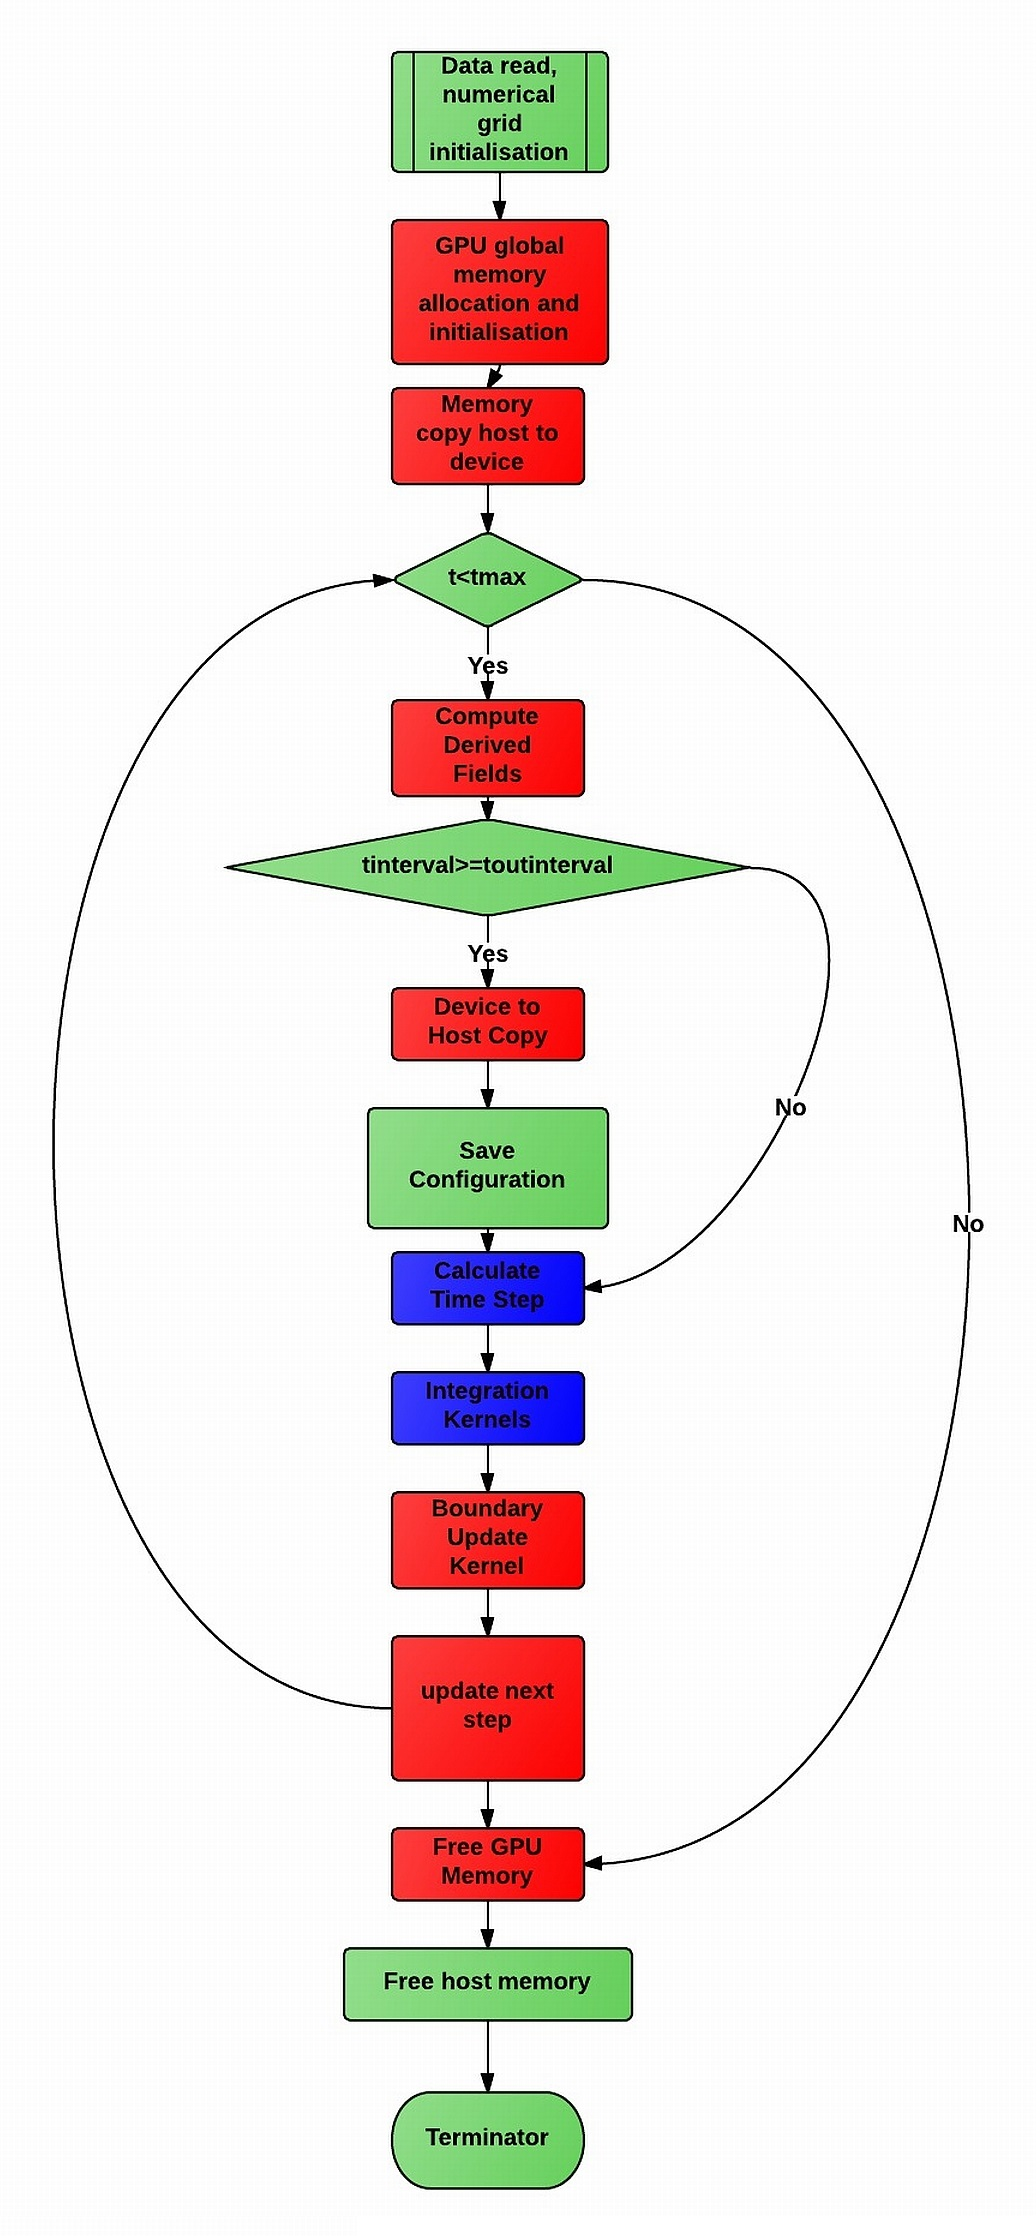
\includegraphics[scale=1.6]{fig1_smaug_mainflow.jpg}
\caption{ Flow diagram for SMAUG,  illustrating the main system elements, kernels running on the GPU are shown in red, routines running on the CPU are shown in green. The blue blocks show units with code which run on both the CPU and GPU.}
\end{figure}



%FIGURE 2 here caption:  Flow diagram for SMAUG,  showing the routines computing the flux updates and hyperviscosity. Kernels running on the GPU are shown in red, routines running on the CPU are shown in Green. The blue blocks show units with code which run on both the CPU and GPU.\\


\begin{figure}[h]
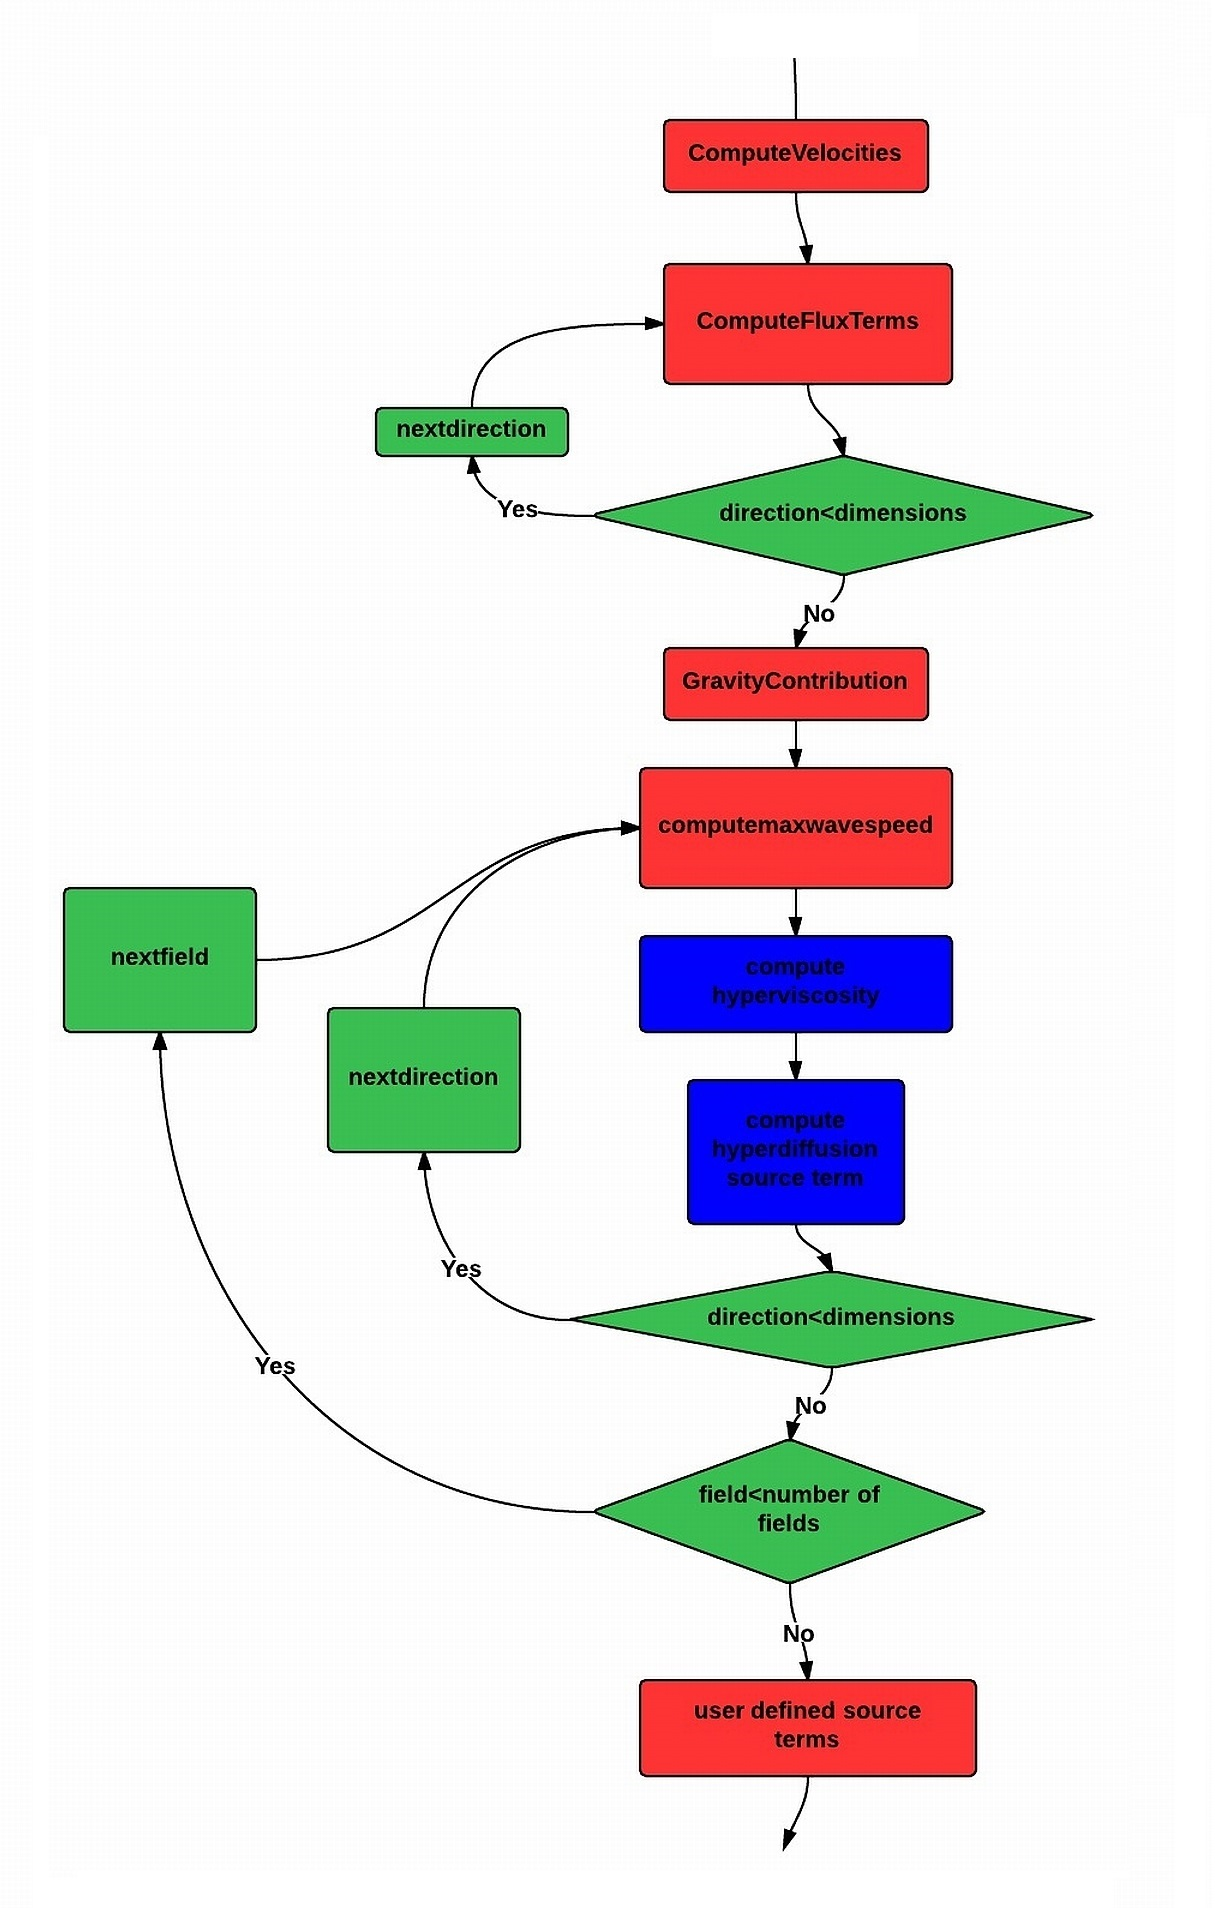
\includegraphics[scale=1.5]{fig2_smaug_integrationkernels-flowdiagram.jpg}
\caption{ Flow diagram for SMAUG,  illustrating the main system elements, kernels running on the GPU are shown in red, routines running on the CPU are shown in green. The blue blocks show units with code which run on both the CPU and GPU.}
\end{figure}












Since the SMAUG frequently refers to a large number of multi-dimensional arrays in one, two or three dimensions, all data is kept in a single 1-dimensional array. We employed an encode routine which converts a 3-dimensional index to a 1-dimensional index. The encode formula is,
\begin{equation}\label{eqindex}
i=i_{1}+i_{2}n_{1}+i_{3}n_{1}n_{2}+f n_{1} n_{2} n_{3}
\end{equation}
where $n_{1},n_{2}$ and $n_{3}$  denote the size of the computation mesh in the $x$, $y$ and $z$ directions respectively. The indices of the mesh point in the  $x$, $y$ and $z$ directions are $i_{1}, i_{2}$ and $i_{3}$ respectively. The index for a particular field component is denoted by  ${f}$. Thus the formula \eqref{eqindex} returns the one-dimensional index for a field point.  A reason for using this data representation is to reduce the number of variables and to reduce the coding required to allow SMAUG to switch between 1D,  2D and 3D geometries.
 With data correctly organised all of the threads within a warp are able to access data within aligned blocks of memory. This behaviour is called memory coalescing \citep{Farber2011}. Memory alignment issues have a significant impact on the utilisation of memory bandwidth and ultimately on performance. For example, the optimal global memory bandwidth is achieved when the threads in a half warp (16 threads) load data from the same memory segment in a single transaction, otherwise performance is degraded as a result of serial accesses to memory. One method of coalescing memory is to allow consecutive threads to access consecutive memory locations. The approach would stagger the updates for each of the field points. It should be noted that, although the M2070 (Fermi) GPU hardware is significantly improved, the issue of coalescing is still a concern. One guideline for ensuring good peformance is to use models whose size scales  as $2^{n}$.

%[Nvidia corporation, CUDA C Programming Best Practices Guides 3.2 August 2011, http://developer.download.nvidia.com/compute/cuda/3_2/toolkit/docs/CUDA_C_Best_Practices_Guide.pdf


% algorithm is required for the computation of the maximum value of a vector of double precision values. 
%Some of the available options are:
%\begin{itemize}
%\item An algorithm using single thread to compare the wave speed to the current maximum value;
%\item A parallel reduction algorithm;
%\item The "atomicMax" function, that treats the maximum value as an atomic value which can only be modified by a single thread at a time;
%\item The "cublasIdamax" function from the CUBLAS library. {cuplaus}
%\end{itemize}
%Unsurprisingly the first, naive algorithm results in an extreme degradation of the algorithm performance. Excellent examples of parallel reduction algorithms are provided by the NVIDIA  "CUDA zone", one of these examples was used as the basis for the reduction algorithm implemented in the SMAUG. 

%Another possibility includes using the "atomicMax" function,
% and the  "cublasIdamax" function from the CUBLAS l
%this treats the maximum value as an atomic value which can only be modified by a single thread at a time.  
The computation of the hyper-viscosity coefficients \eqref{eqhyp} requires the calculation of the maximum wave speed in the computational domain. An interleaved addressing method was used for the computation of the maximum value of a vector of double precision values of the maximum wave speed. Figure 3 illustrates the interleaved addressing method for parallel reduction. The example illustrated here is a global summation. The sum of data items accessed by adjacent threads is evaluated. At the first step every other thread is used to compute part of the reduction, as further steps are taken the stride is doubled. This algorithm results in a significant enhancement in the performance.  As discussed earlier, shared memory is much faster than global memory, so the parallel reduction algorithm benefits greatly.\\


%FIGURE 3 here caption:Illustration of the interleaved addressing method for parallel reduction.\\


\begin{figure}[h]
%%\includegraphics[scale=0.25]{figure1.jpg}
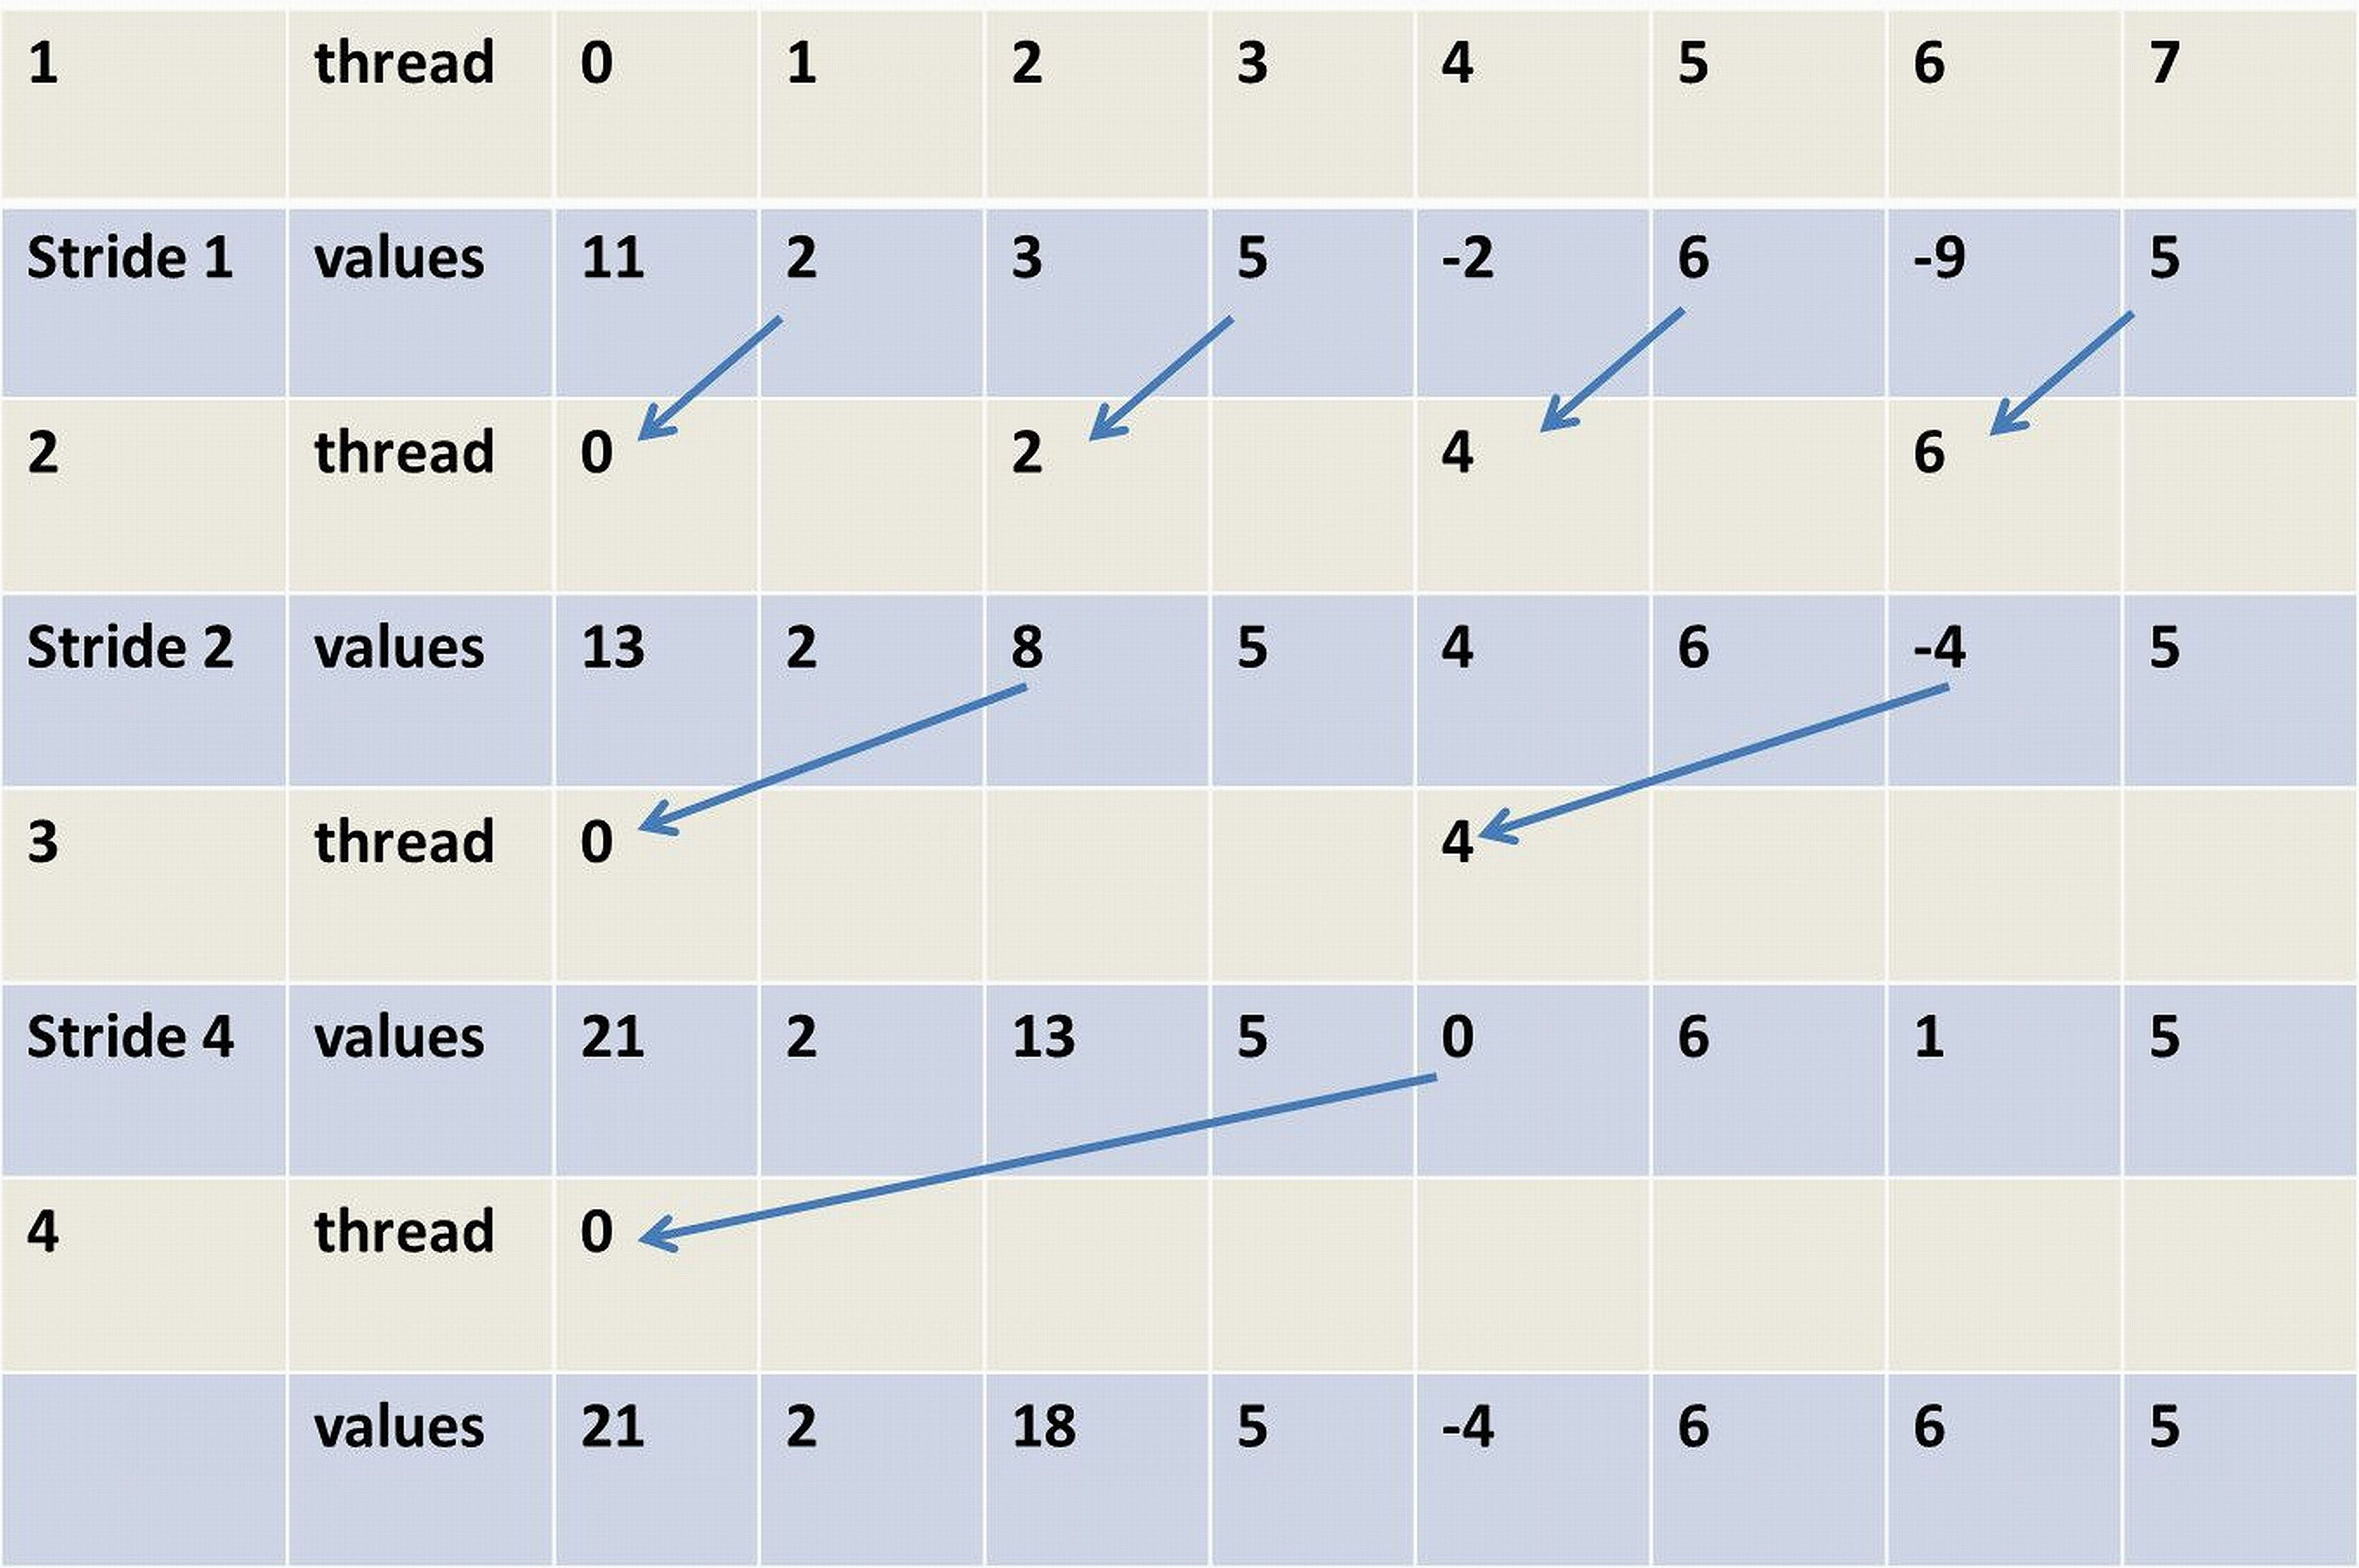
\includegraphics[scale=0.5]{figure3.jpg}
\caption{Illustration of the interleaved addressing method used for parallel reduction.}
\end{figure}


 Figures 4  and 5 show code segments from the reduction algorithm used to compute the wave speed maximum. Figure 4 illustrates how the interleave method is applied to each of the thread blocks. It is necessary to call the available number of threads per block to determine the size of the GPU shared memory required to store and compare the wave speeds for this computation. By accessing shared memory we take advantage of the greater GPU data bandwidths. After the execution of all of the thread blocks a single loop is used to obtain the required maximum value. Figure 3 shows the kernel  for the reduction  routine; the first part allocates the shared memory and transfers data from the GPU global memory. The interleave
method is implemented by the section of enclosed by comments indicating the start and end of the repeating code block. The final line of the segment writes the partial value for the first thread and stores the maximum values for each of the thread blocks.\\ 

%FIGURE 4 here caption:Host code used to call reduction routine CUDA kernel. The start of the section shows the initialisation of the shared memory size and the number of threads per block. The middle section shows the allocation of CUDA device memory used to store the maximum values for each thread block. The final section calls the CUDA kernel, determines the maximum value for the %thread blocks and writes the global maxima (for all thread blocks)  this resulting value is finally copied to the device memory.\\

%FIGURE 5 here caption:CUDA kernel implementation of the interleave method for the reduction algorithm. The first part of the kernel initialises the shared memory for each thread block. The array of shared memory values is set with the wave speed values stored in the GPU memory. The interleave operation can only perform after synchronisation of the threads for each block. The repeating %segment of code which follows is the interleave operation each thread even numbered thread compares a pair of values in the shared memory. The reduction occurs as the repetition strides over each set of neighbouring values. Before each stride can commence it is necessary for all the threads in the block to be synchronised. The nature of this reduction operation is such that the required %value is stored in the first memory location in the array, this result in shared memory is transferred to the array of results for each of the thread blocks.\\

For the computation of the fluxes and hyper-diffusion terms, we expect the performance to scale as $N^{2}$, this is due to the fact that we can map each thread to an element of the computational mesh. In the case of the reduction operation the performance for techniques such as the interleave method scales as $N \ln N$. This provides a limit for the speed-up which may be achieved by SMAUG.

\begin{figure}[h]
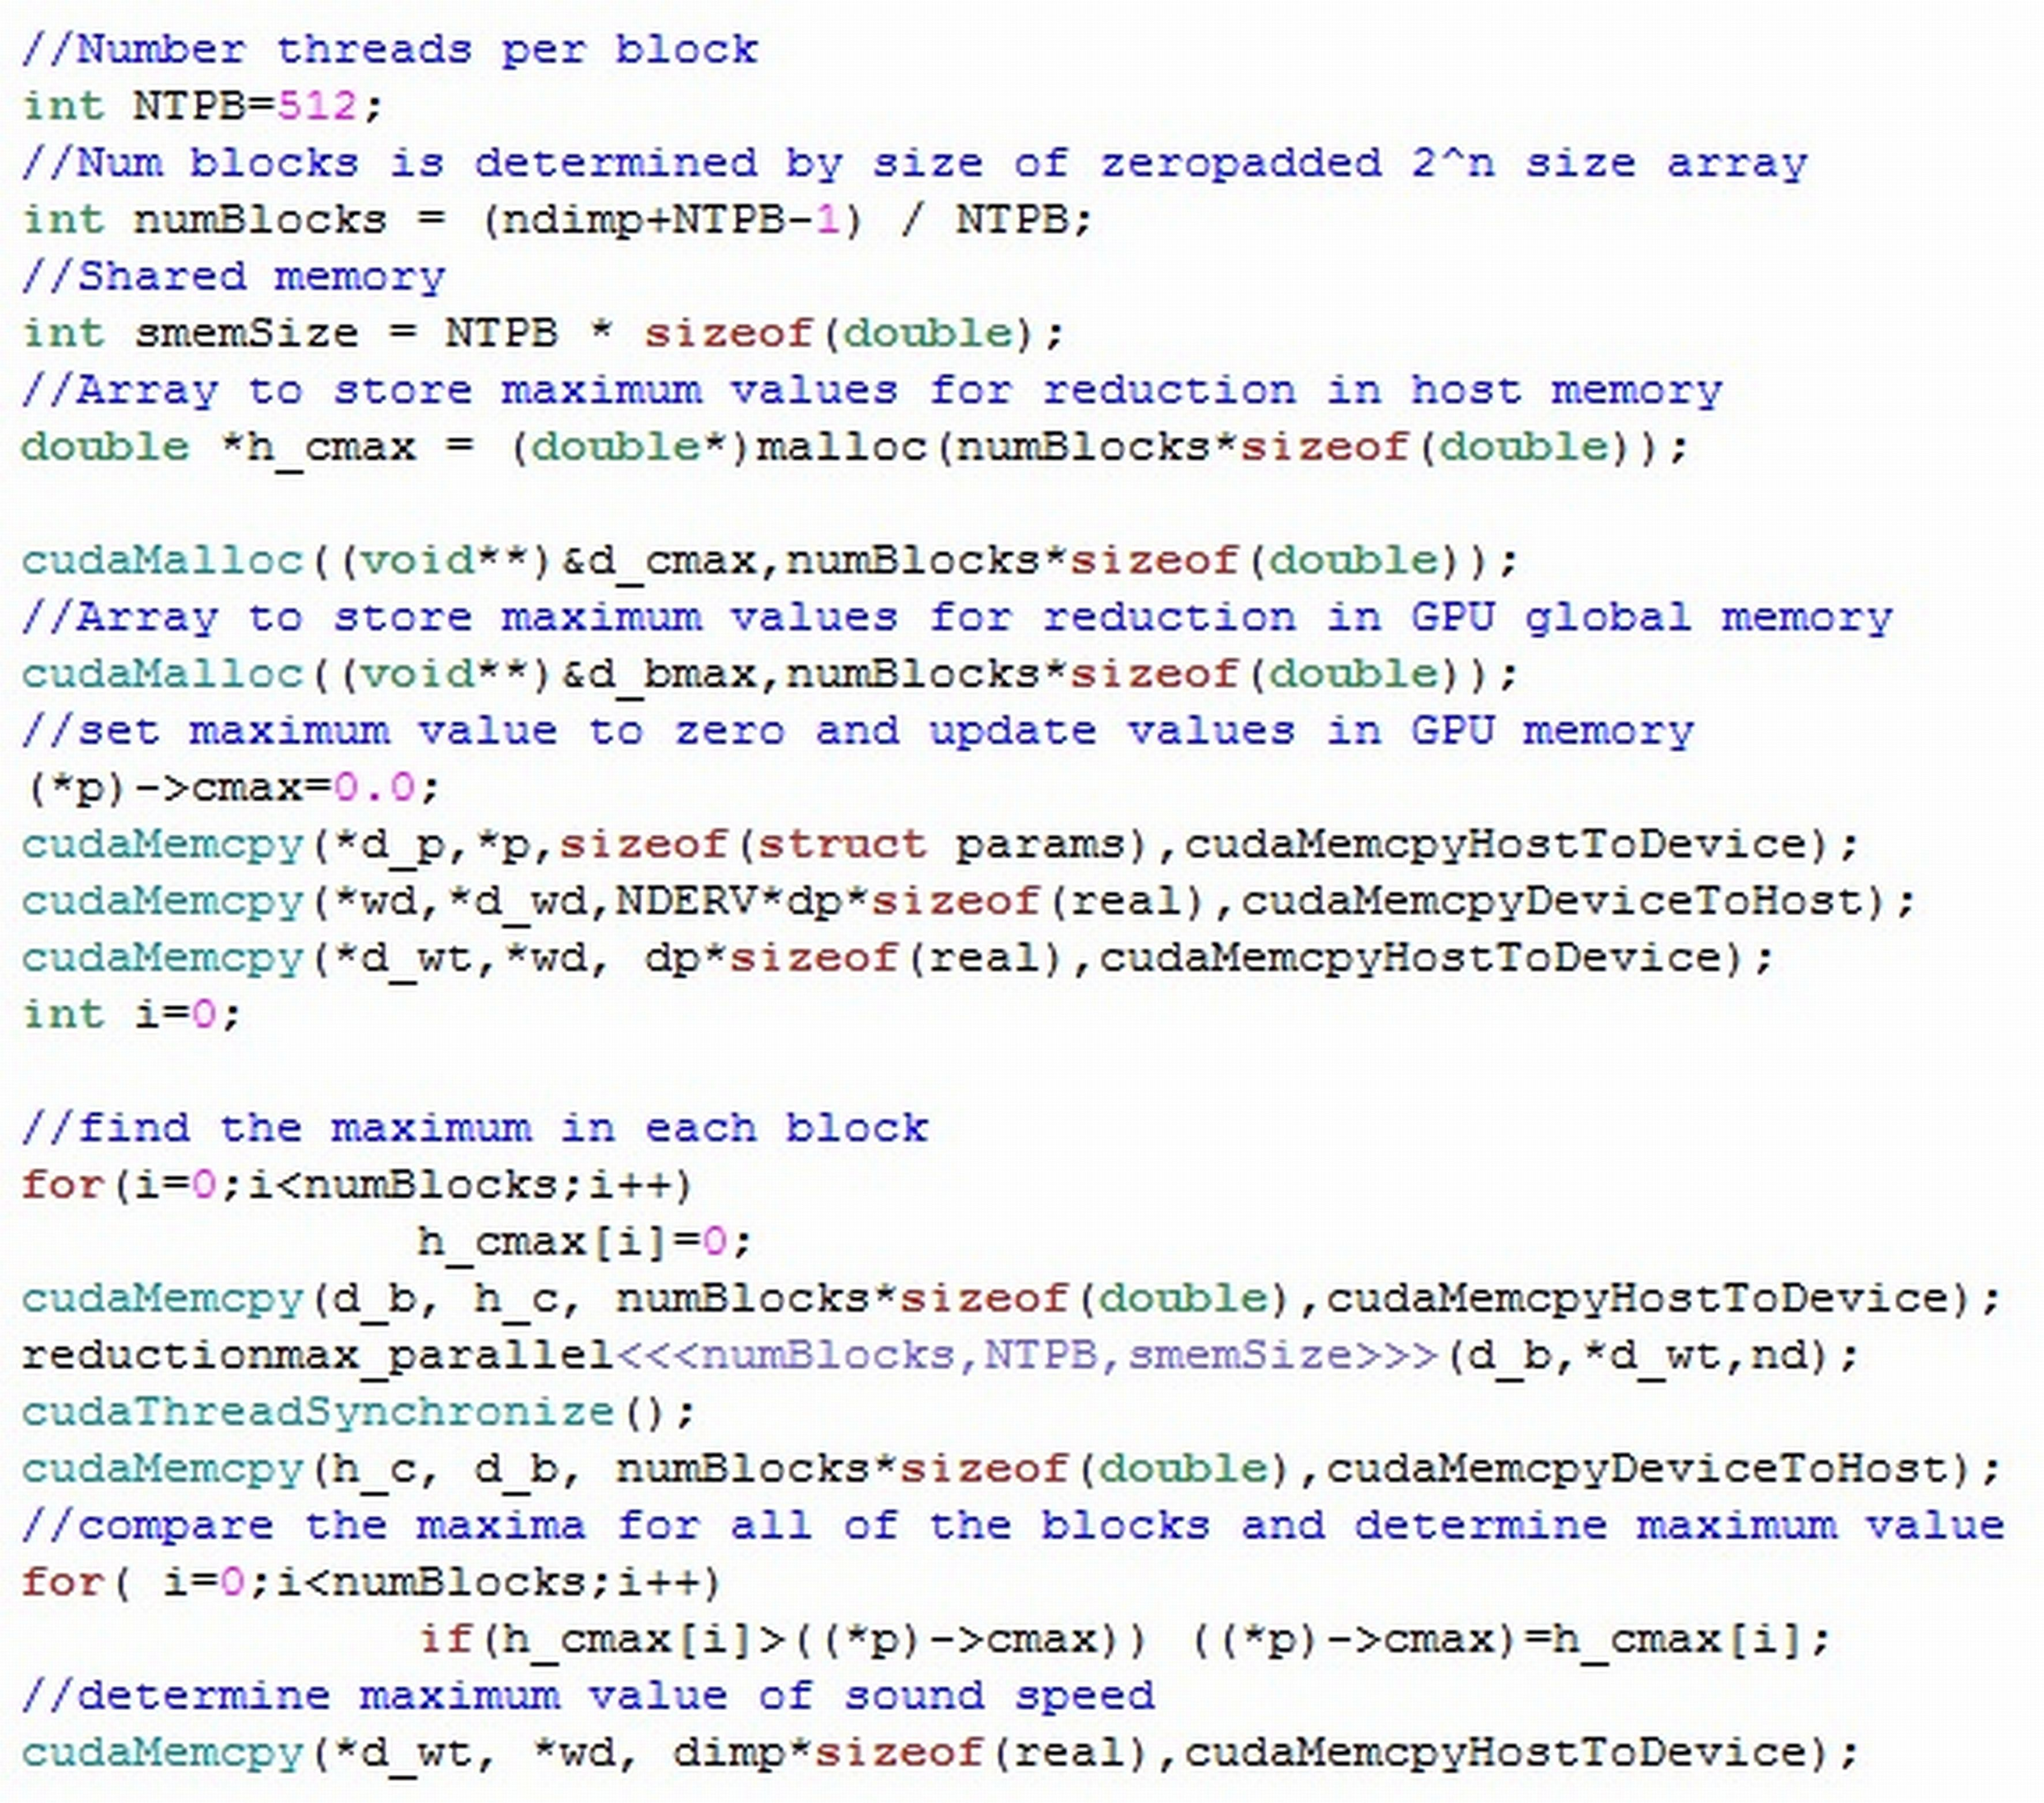
\includegraphics[scale=0.75]{cucomputemaxc_fig4}
\caption{Host code used to call reduction routine CUDA kernel. The start of the section shows the initialisation of the shared memory size and the number of threads per block. The middle section shows the allocation of CUDA device memory used to store the maximum values for each thread block. The final section calls the CUDA kernel, determines the maximum value for the thread blocks and writes the global maxima (for all thread blocks)  this resulting value is finally copied to the device memory. }
\end{figure}

\begin{figure}[h]
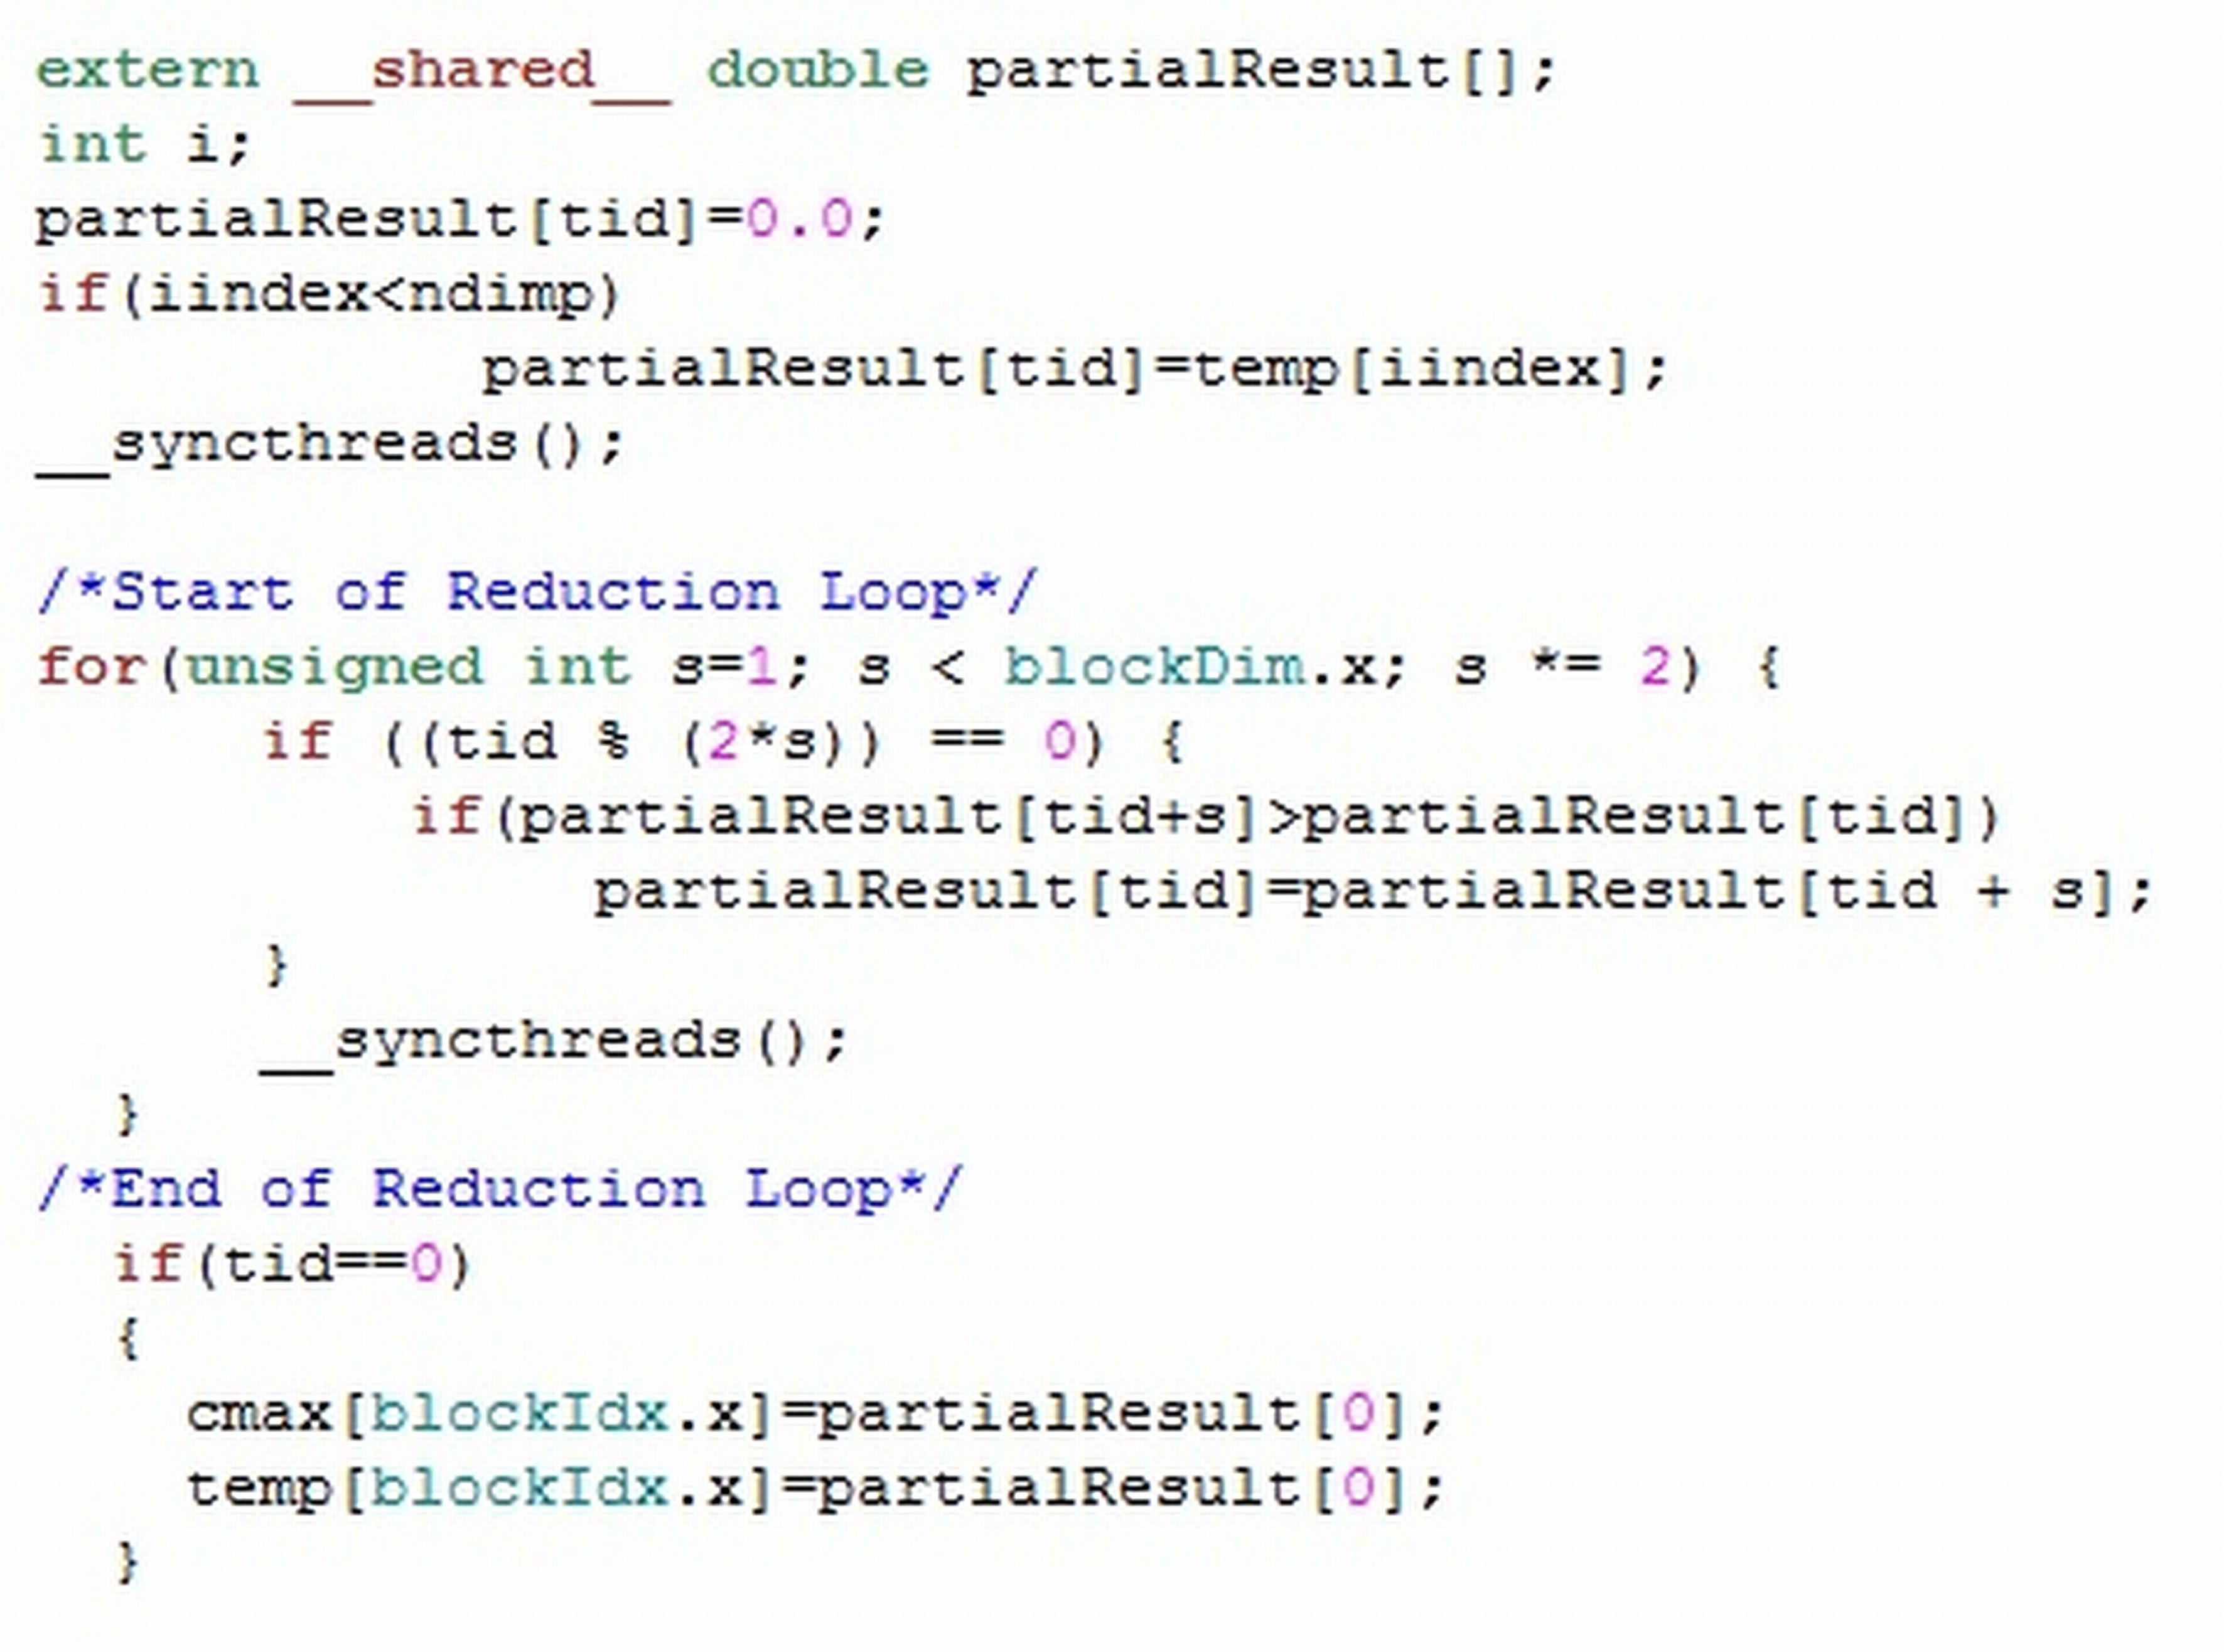
\includegraphics[scale=0.75]{reduction_parallel_fig5.jpg}
\caption{CUDA kernel implementation of the interleave method for the reduction algorithm. The first part of the kernel initialises the shared memory for each thread block. The array of shared memory values is set with the wave speed values stored in the GPU memory. The interleave operation can only perform after synchronisation of the threads for each block. The repeating segment of code which follows is the interleave operation each thread even numbered thread compares a pair of values in the shared memory. The reduction occurs as the repetition strides over each set of neighbouring values. Before each stride can commence it is necessary for all the threads in the block to be synchronised. The nature of this reduction operation is such that the required value is stored in the first memory location in the array, this result in shared memory is transferred to the array of results for each of the thread blocks. }
\end{figure}






SMAUG consists of a collection of  3 source files for code that runs on the host system and 23 kernel source files for code that executes on the GPU. Using conditional compilation through the compiler preprocessor, the code has a degree of flexibility and provides a number of defined preprocessor variables which may be altered within an input file used by the $\it{make}$ routine. The optional preprocessor variables enable switching between 1D, 2D or 3D geometries, running across multiple GPUs, user-provided source terms or switching between double and single precision.





SMAUG was developed using a Waterfall software engineering methodology, see \citep{Pressman 1997}. SMAUG is licensed under the GNU General Public License (GPL v3.0). The decision to make SMAUG freely available should ensure that the software will always be available and should encourage the user community to extend  and to accelerate new scientific and algorithmic developments. SMAUG is available at
\\ 
\href{https://code.google.com/p/smaug/}{https://code.google.com/p/smaug/}.
\\






An important consideration for SMAUG is its inter-operability with the existing SAC code. For this reason SMAUG has been deliberately designed to read and write configuration files generated by the SAC initialisation routines. The distribution routines are used to scatter and gather configuration files for use in MPI enabled problems.IDL and Matlab visualisation routines already used with SAC and VAC may be re-used. The source distribution provides a number of sample problems which are configured using the $\it{make}$ routine. Verification tests have been performed to verify the results generated by SMAUG and to assess the performance. Results are discussed in the following two sections.

\section{Verification Tests}

A challenge for solving hyperbolic differential equations such as the MHD equations  \eqref{eqprho}-\eqref{eqppkb}  arises when solutions are sought for systems exhibiting discontinuities in their solution.  A number of tests have been performed in 1D, 2D and 3D geometries. Such tests are crucial for ensuring the robustness of  the solver. We verified that SMAUG reproduces the same results as SAC for the Brio-Wu, Orszag-Tang, a 3D blast-wave problem and a 3D model of wave propagation in a gravitationally stratified solar atmosphere. Details of the first three standard tests are given in Appendix B.
One of the objectives of the tests is to ensure the correct implementation of the hyper-diffusion algorithm for stabilising the solutions from numerical instabilities.

 To isolate algorithmic differences we ran both codes with the hyper-diffusion switched off. As the agreement between SAC and SMAUG was progressively improved, each of the hyper-diffusion contributions was tested in turn. For example, testing would be undertaken with just the hyper-diffusion contribution for the density enabled. Finally, all of the hyper-diffusion  source terms were included. The percentage difference between SAC and SMAUG for the total density and total energy for the Orszag-Tang test is shown in Figure 6. To understand the differences observed in Figure 6  we performed a number of experiments using the Orszag-Tang test. As well as comparing results generated using SAC and SMAUG we compared the difference between results for SAC and SMAUG when a small error in the density was introduced at the centre of the numerical grid. The magnitude of the introduced difference was at the level of the round off error. These experiments resulted in deviations in the total energy and momentum which were of the same order of magnitude as those presented in Figure 6. It is well understood that NVIDIA GPUs are fully compliant with the IEEE-754 standard for floating point operations, see \citep{Whitehead 2011}. Differing computer processor architectures can lead to numerical differences when performing a computation with a large number of operations which may have large differences in magnitude.\\





%FIGURE 6 here caption: Percentage difference between SAC and SMAUG calculation of total energy and total density at each iteration for the Orszag-Tang vortex problem computed on a 256x256 numerical grid.\\
\begin{figure}[h]
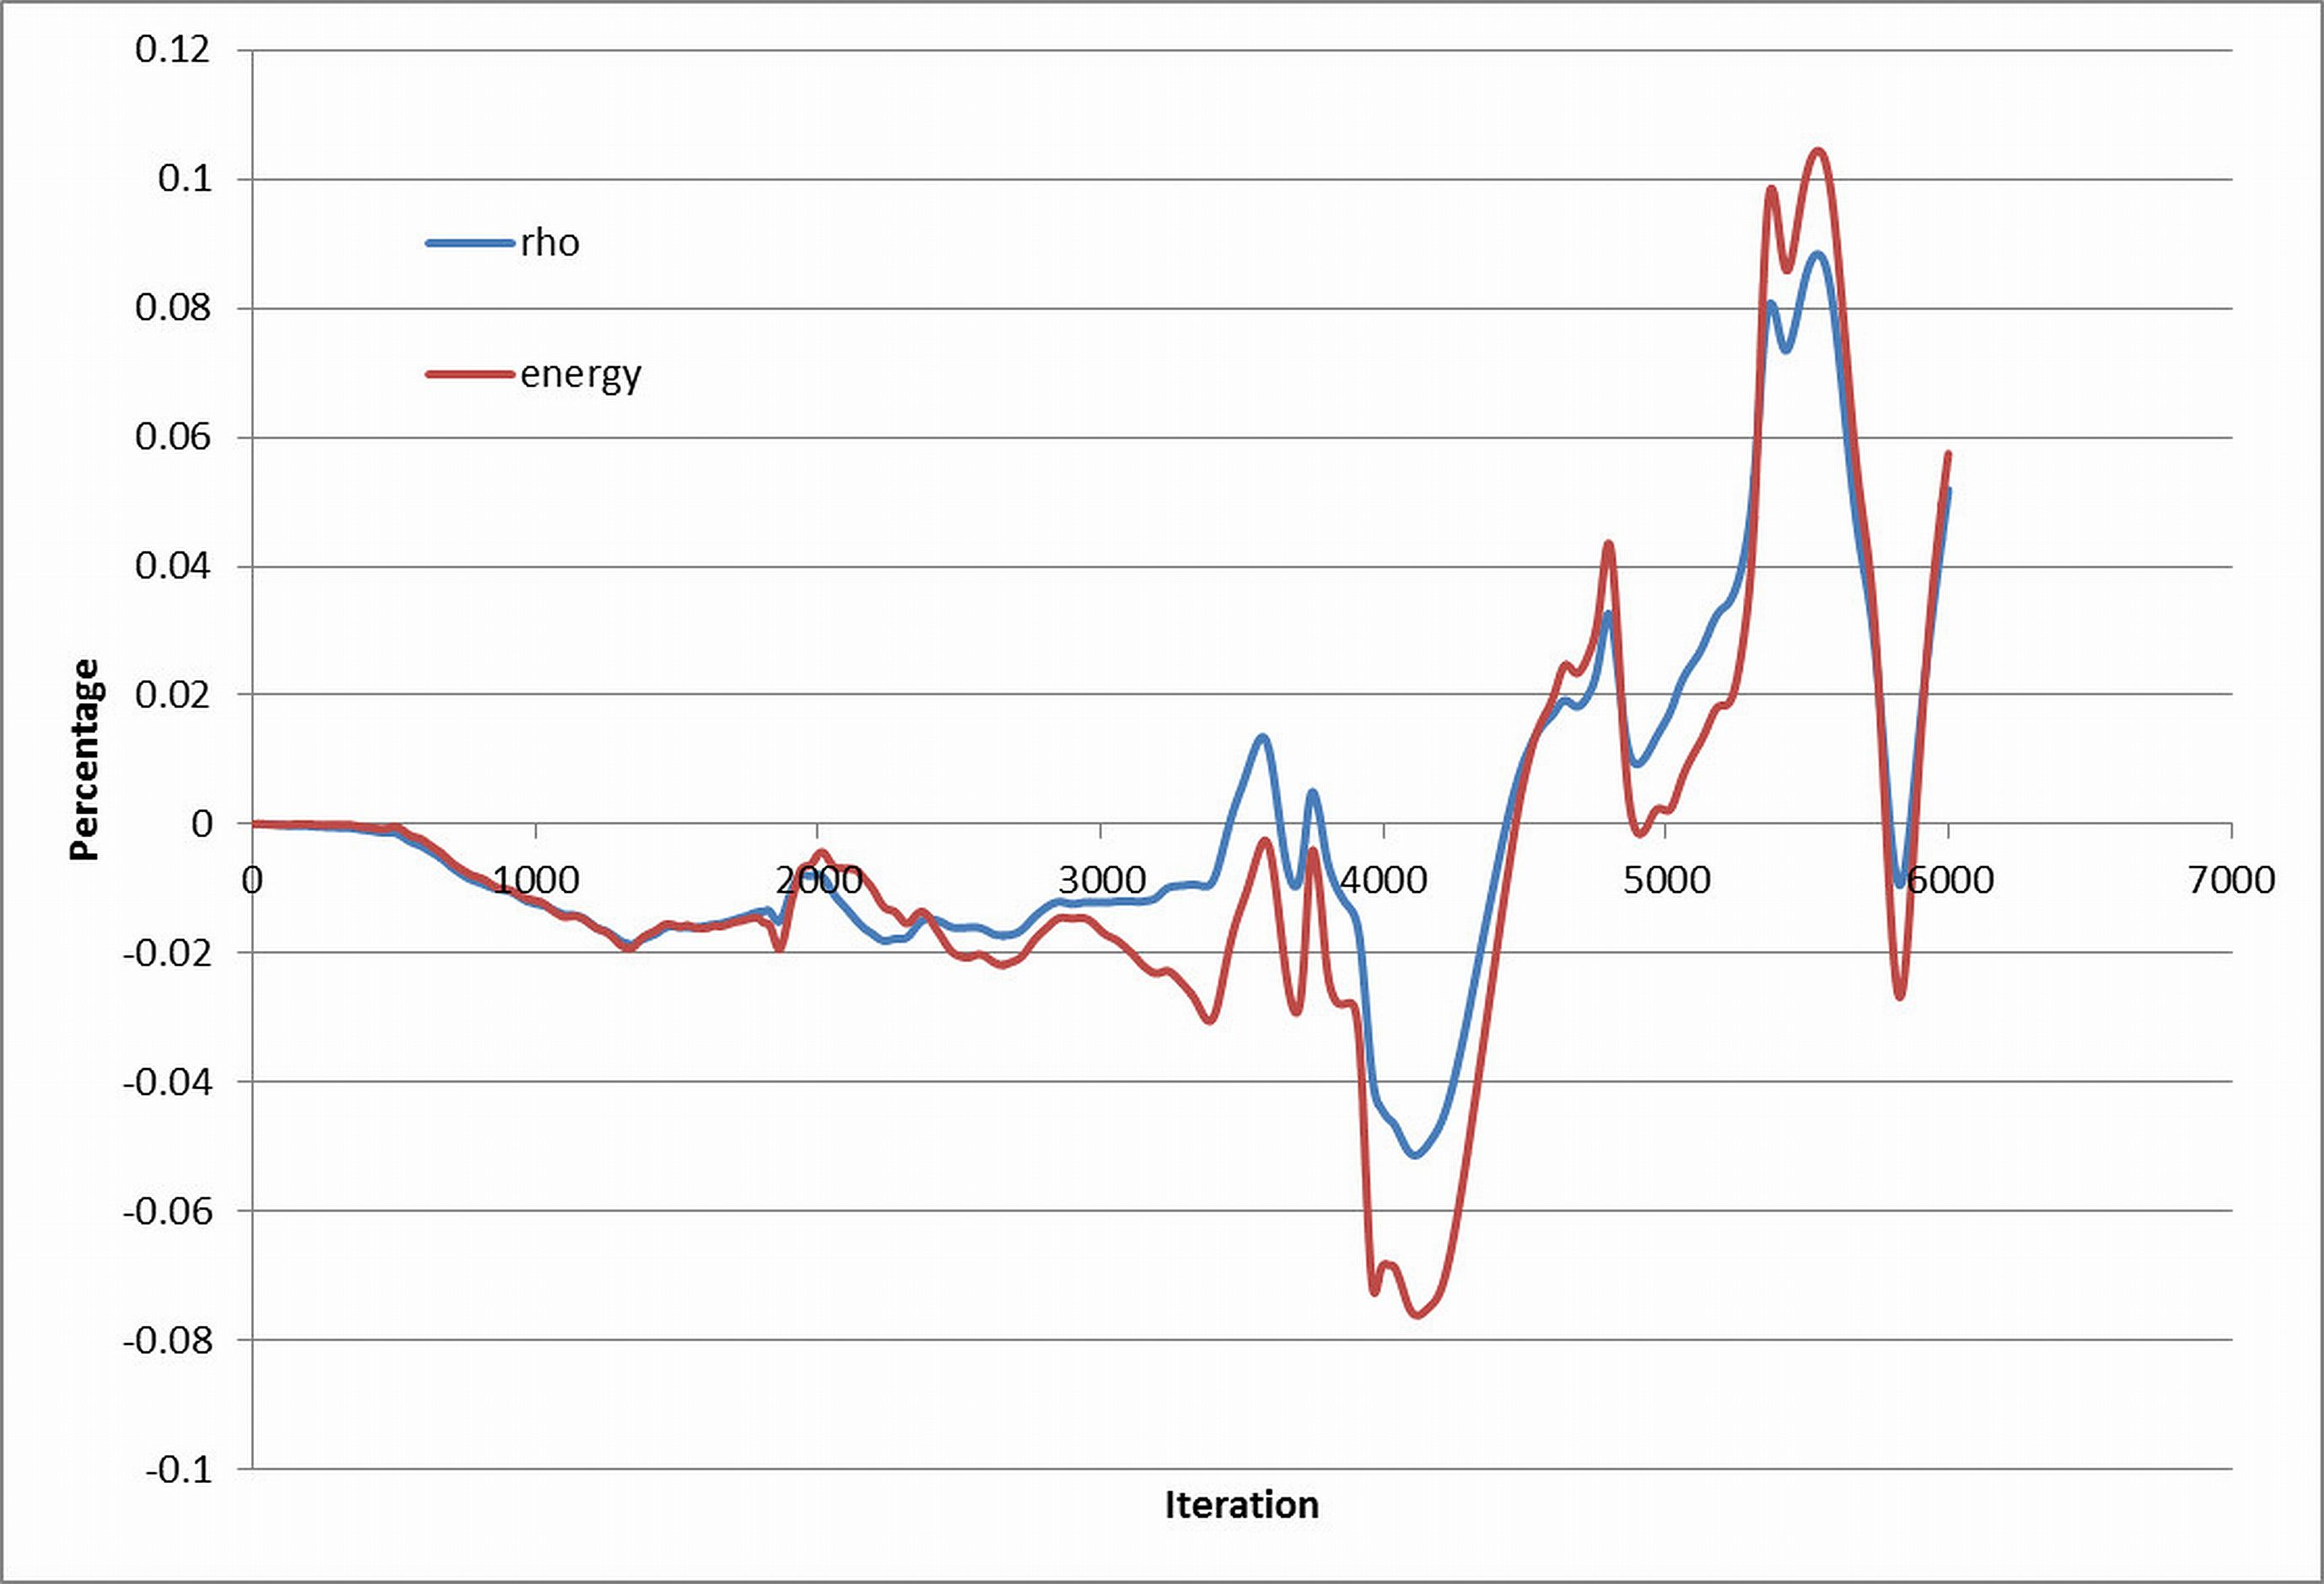
\includegraphics[scale=0.9]{figure6_percentenergydensitydifference_ozt_sacsmaug_tp5.jpg}
\caption{Percentage difference between SAC and SMAUG calculation of total energy and total density at each iteration for the Orszag-Tang vortex problem computed on a 256x256 grid.}
\end{figure}


%{ Differences between the results from the two algorithms are not just algorithmic differences or coding errors but may be attributed to the  ordering of IEEE-754 floating-point operations which are not associative. Computation of the hyper-diffusion terms requires the ordering %of large numbers of operations (i.e. summations) handling operands which have substantially different magnitudes.  Villa et al. %\citep{Villa2008} point our that this effect may be exacerbated in multithreaded computations where interleaving of floating point operations is non-deterministic and results in non-deterministic numerical error propagation. The approach of  Villa et al. \citep{Villa 2008} is to  %enforce parallel deterministic operations at compile time for highly multithreaded architectures. 
%}


 

%\clearpage
\subsection{MHD Wave Propagation in Magnetised and Gravitationally Stratified 3D Solar Atmosphere}

In this section we provide the numerical results of modelling of MHD wave propagation in an open magnetic flux tube embedded in the solar atmosphere. The background model and initial setup of the problem are similar to used previously in \citep{Fedun et al. 2011, Fedun et al. 2011c, Fedun et al. 2011b}. This simulation examines SMAUG's capability for modelling the physical processes in the magnetized and stratified media expanding from the photosphere through chromosphere, transition region and into the solar corona.


It is planned to use SMAUG for modelling the physical processes of the magnetically coupled solar interior and atmosphere. Work is also in progress to study the propagation of energy into the solar atmosphere  by using a vibrating membrane to drive the lower boundary of the simulation box. Such studies provide insight into the coupling of the solar global eigenmodes with motions in the solar atmosphere. 

Here we present initial results for modelling of MHD waves in a chromospheric magnetic flux tube. The problem tests SMAUG's capability for modelling a gravitationally strongly stratified 3D solar atmosphere. Vortex motion at the foot point of the magnetic flux tube is excited by the a time-dependent torsional driver (see \citep{Fedun et al. 2011, Fedun et al. 2011c, Fedun et al. 2011b}), we used a velocity amplitude of 20 m/s with no time-dependence for the driver. An additional model was repeated with the velocity amplitude set to 200 m/s and the period of the driver set to 120s.  In Figure 7 we have shown a 2D vertical cross-cut through the 3D numerical domain for the $\it V_{y}$ velocity component. \citep{Mumford et al. 2014} are using SMAUG in a study of the effect of photospheric motions on the generation of MHD Waves in low solar atmospheric flux tubes. 



%FIGURE 7 here caption: The vertical cross-cut through the 3D numerical domain. Snapshots of the $V_{y}$ component of the velocity  response showing the temporal evolution of the initial  perturbation  generated by 120 s period torsional driver  at t=32, 64, 96 and 128 s  in the open magnetic flux tube respectively. The color scale shows the $V_{y}$ perturbations in km/s. For more details %of mathematical set-up of this physical problem consult  \citep{Fedun et al. 2011}\\

\begin{figure}[]
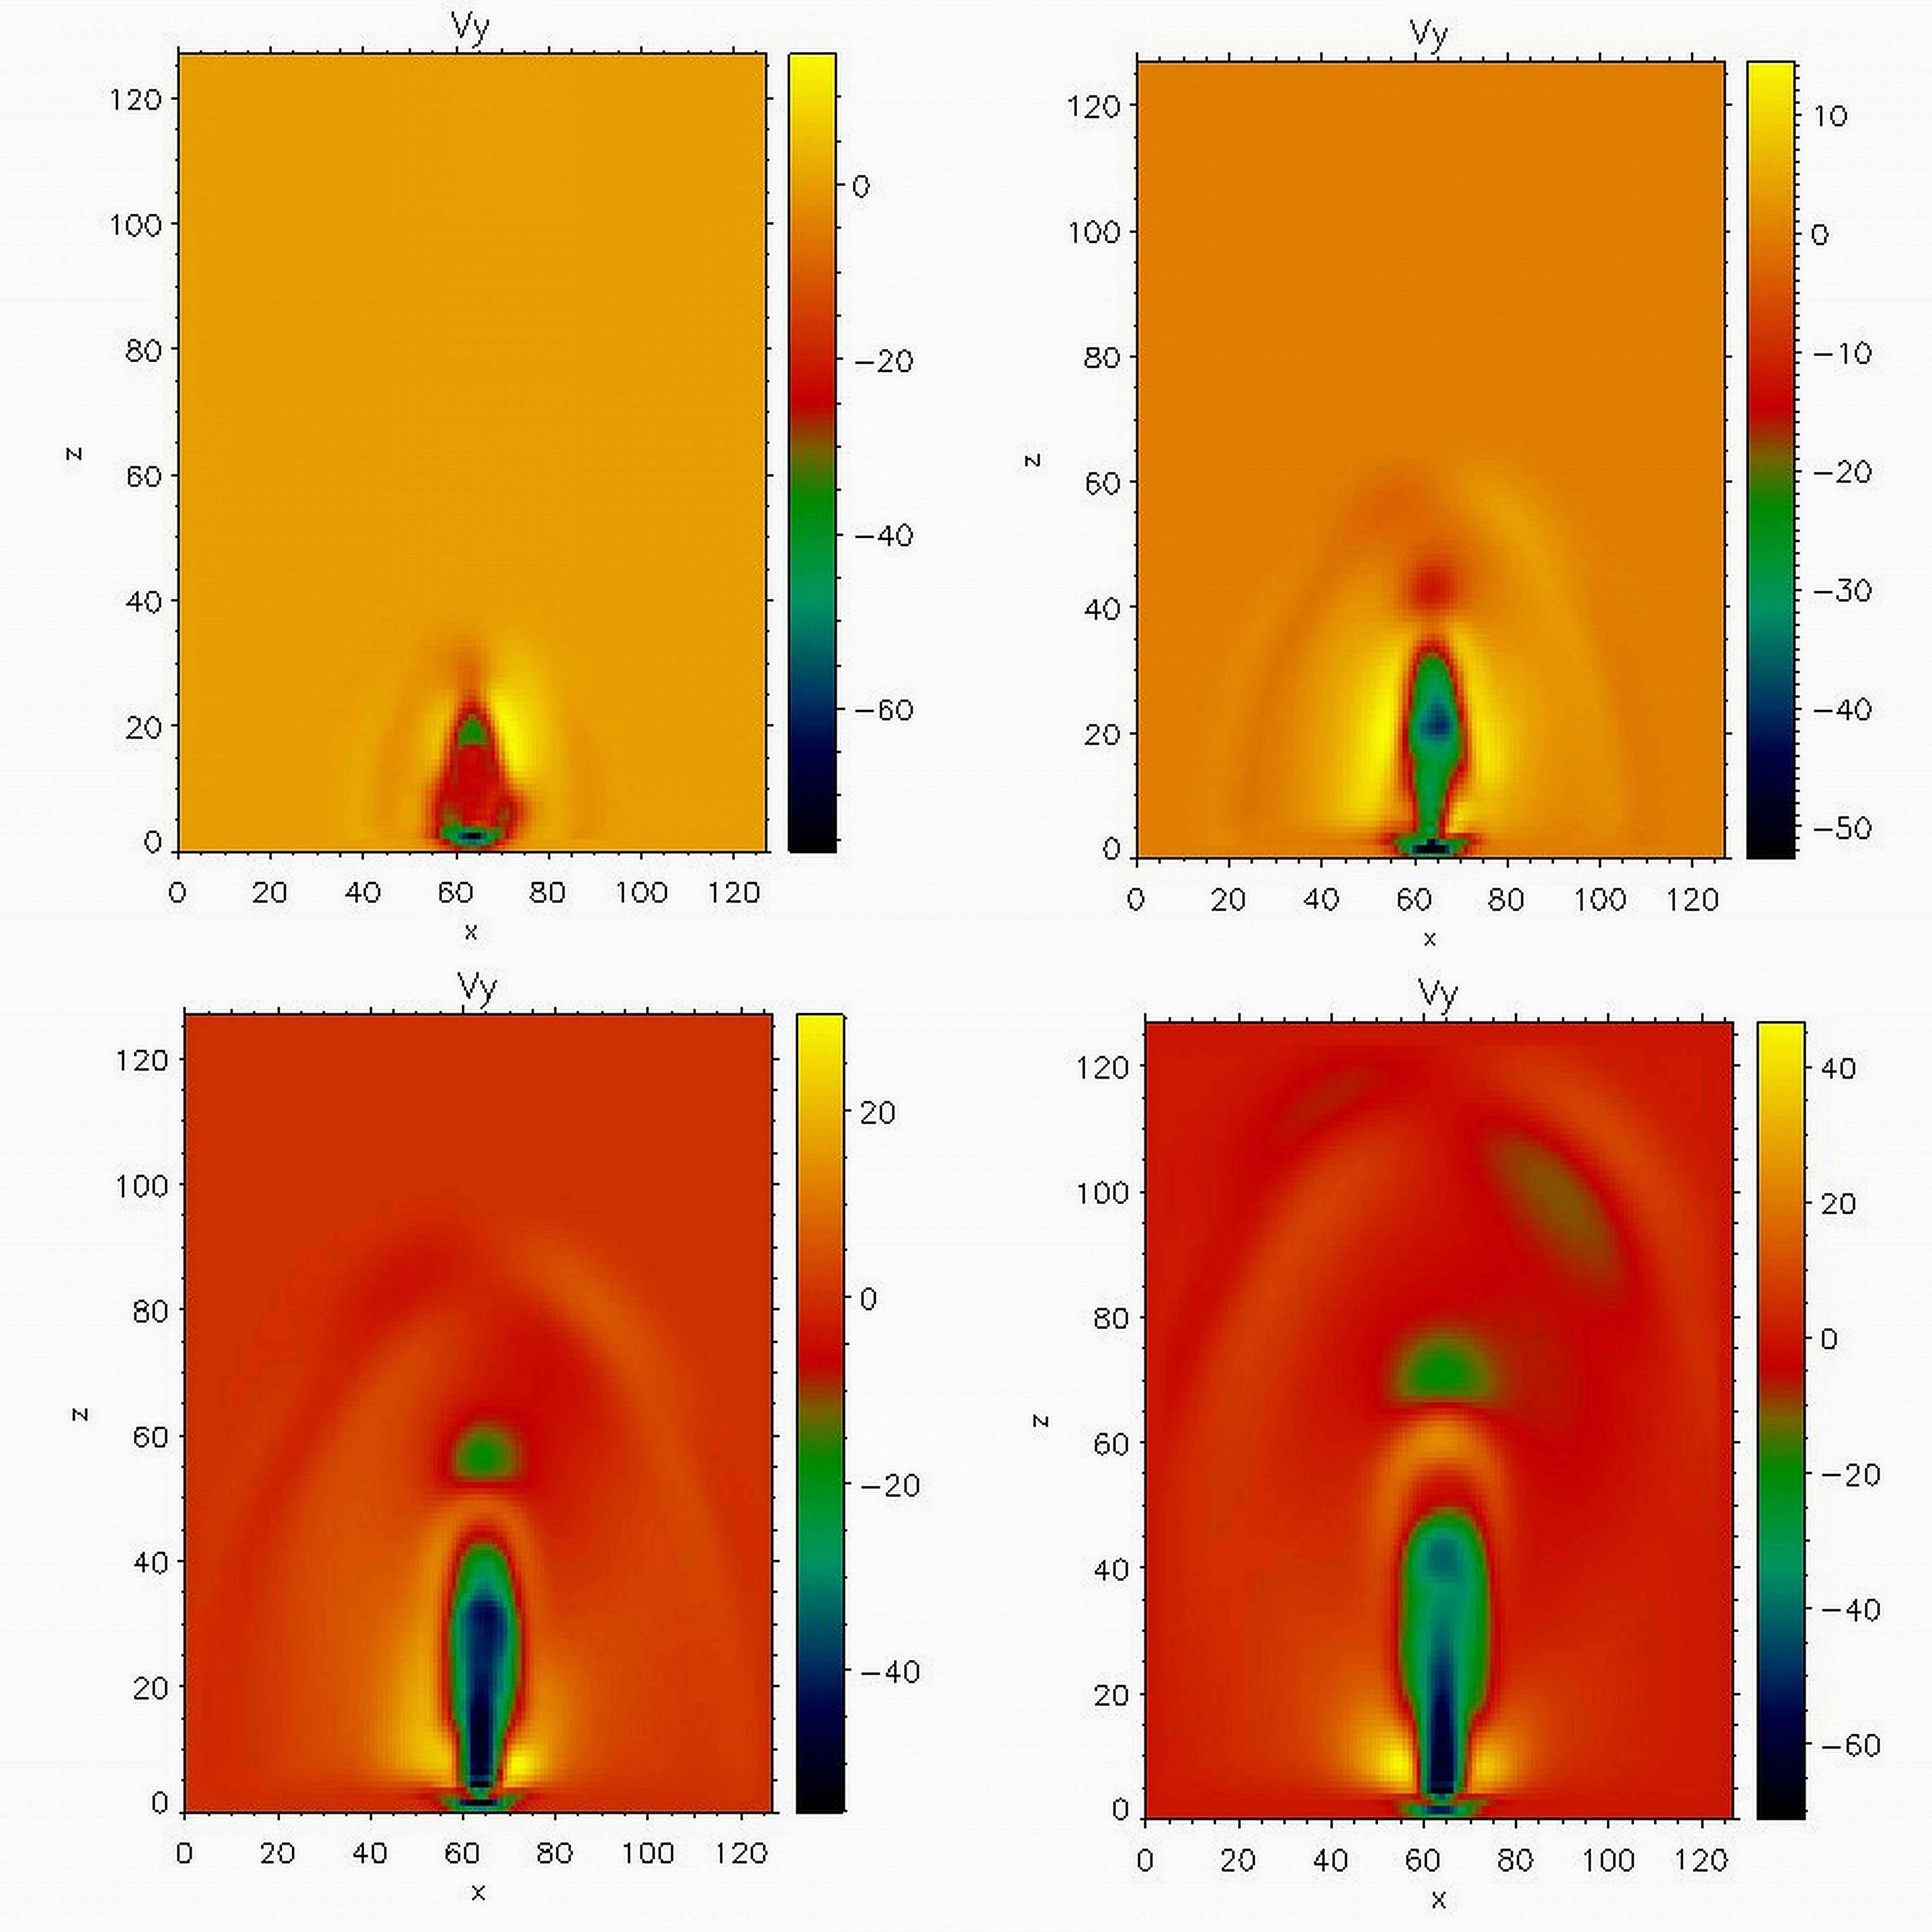
\includegraphics[scale=1.0]{figure7_fluxtube.jpg}
\caption{The vertical cross-cut through the 3D numerical domain. Snapshots of the $V_{y}$ component of the velocity  response showing the temporal evolution of the initial  perturbation  generated by 120 s period torsional driver  at t=32, 64, 96 and 128 s  in the open magnetic flux tube respectively. The color scale shows the $V_{y}$ perturbations in km/s. For more details of mathematical set-up of this physical problem consult  \citep{Fedun et al. 2011}}
\end{figure}



%\clearpage
\section{Performance Measurements}

The performance of SAC and SMAUG was assessed by running the Orszag-Tang problem for varying problem sizes on Intel Xeon (X5650 CPU (6 cores, 2.67GHZ clock frequency), E5 2670 CPU (8 cores, 2.6GHz)) and GPU NVIDIA (C1060 (Tesla), M2070 (Fermi), K20 (Kepler)) computer architectures.

The NVIDIA GPU device architecture and programming methodology was described in Section 2. For all of the CPU tests, SAC was compiled using the Portland Fortran90 compiler version 10.2 with full optimisation. For the CPU runs the problems were initially run using a single processor core. Figure 8 and 9 show comparisons of the computational time taken to perform 100 iterations with a varying grid size for each of the processors. Figure 8 and 9 compare the timings for the Intel X5650  and Intel E5-2670 CPU respectively. The result clearly indicates that as the grid size increases, both the C1060 and M2070 GPUs offer significant improvement in the time taken to complete an iteration. This is the initial evidence that the GPU performance scales well with grid size. 

To obtain a better understanding of the performance benefits of running the problem on a GPU, we compare the speed-up factor for the C1060, M2070 and K20 GPUs for each of the tested CPUs. Defining $t_{c}$ as the time to complete 100 iterations on the CPU and $t_{g}$ as the time to complete 100 iterations on the GPU; the speed up factor is defined as ${t_{c}}/{t_{g}}$. Figure 10 and 11 show the speed-up factor versus the model numerical size comparing C1060, M2070 and K20 against the Intel Xeon X5650 CPU and Intel Xeon E5-2670 CPU respectively.  The C1060 offers a speed up of 4 over the Intel Xeon X5650 CPU, in contrast to the M2070 GPU, we observe that this benefit does not improve with increasing the problem size. This may be understood in terms of the enhanced double precision performance for the M2070 GPU. This is a result of the higher memory bandwidth achieved for double precision values. One of the reasons for the enhanced performance with increased problem size is due to the number of threads assigned to the cores. Increasing the occupancy in this way hides some of the effects of memory latency in transferring data from the GPU global memory to the block memory. The results demonstrate that for the NVIDIA K20 the SMAUG achieves a speed-up of up to 18 times when compared to a single Intel Xeon X5650 processor core, such a speed-up is achieved for problem sizes which fully occupy the GPU. 

In Figure 12 and 13 we present  the performance for the GPUs against fully occupied Intel CPUs figure 12 compares the speedup acheived using a fully occupied 6 core Intel Xeon X5650 CPU and Figure 13 compares the speedup achieved compared to the 8 core Intel Xeon E5-2670. The results shown in Figures 12 and 13 display a characteristic dip for moderate levels of the problem size. This dip results from the performance for the CPU, at this domain size the multicore CPU benefits from optimal utilisation of CPU cache memory. The performance comparison with multi-core CPUs is dependent on the decomposition of the problem across the multicore processor we will return to this issue when SMAUG is distributed across multiple GPUs. We note, however, that the C1060 GPU is still able to offer significant performance enhancement compared to the Intel Xeon X5650 CPU. Using the Kepler K20 we have acheived a speedup of factor 3 compared to a fully occupied Intel Xeon E5-2670 CPU.

It was pointed out that the performance of the algorithm scaled as $N\ln{(N)}$, this arises from the reduction operation used by the computation of the maximum wave speed. Application profiling indicates that the computation of the boundary conditions does not provide a significant contribution to the acceleration of the algorithm. This is due to the limited quantity of data used in the update process. As indicated in the results it was observed that the GPU performance improved as the problem size was increased. A further issue with the computation of the boundary terms is due to the non-coalescent memory access.\\


%FIGURE 8 here caption: Comparison of the run times for 100 iterations of the Orszag-Tang problem. The run times obtained with the Intel X5650 processor and different NVIDIA GPUs and with varying problem sizes are shown.\\

\begin{figure}[h]
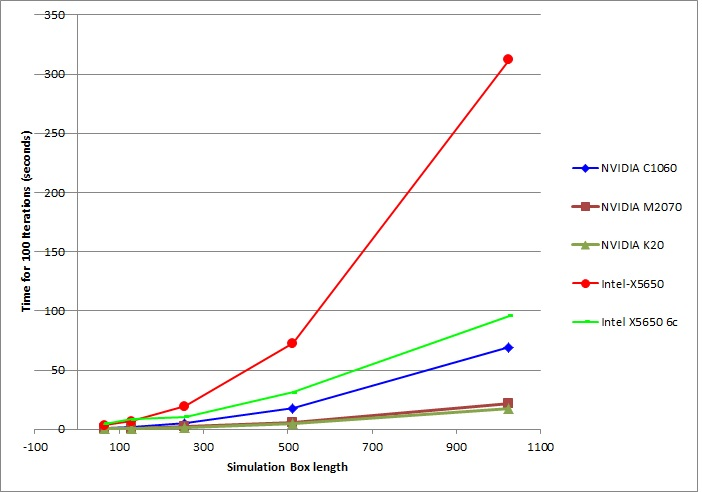
\includegraphics[scale=0.7]{figure8_x5650_timings.jpg}
\caption{Comparison of the run times for 100 iterations of the Orszag-Tang problem. The run times obtained with the Intel X5650 processor and different NVIDIA GPUs and with varying problem sizes are shown.}
\end{figure}



%FIGURE 9 here caption: Comparison of the run times for 100 iterations of the Orszag-Tang problem. The run times obtained with the Intel E5-2670 processor and different NVIDIA GPUs and with varying problem sizes are shown.\\

\begin{figure}[h]
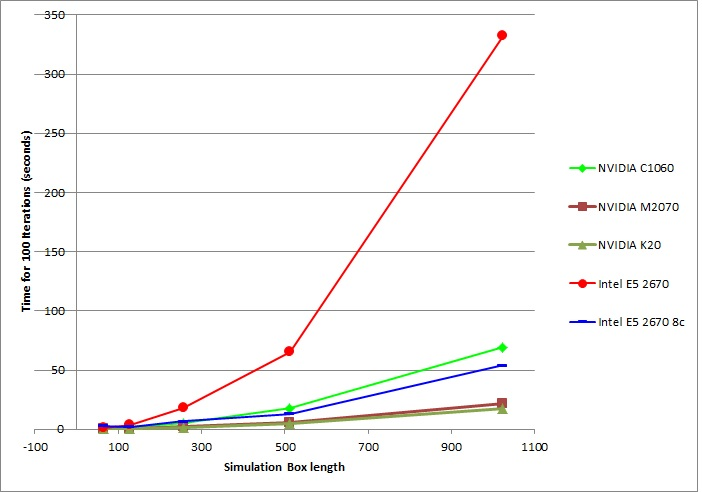
\includegraphics[scale=0.7]{figure9_e52670_timings.JPG}
\caption{Comparison of the run times for 100 iterations of the Orszag-Tang problem. The run times obtained with the Intel E5-2670 processor and different NVIDIA GPUs and with varying problem sizes are shown.}
\end{figure}




%FIGURE 10 here caption: Measured speed up factors for the Orszag-Tang test problem performed on different numerical grids, comparing NVIDIA GPUs against the Intel X5650 CPU.\\

\begin{figure}[h]
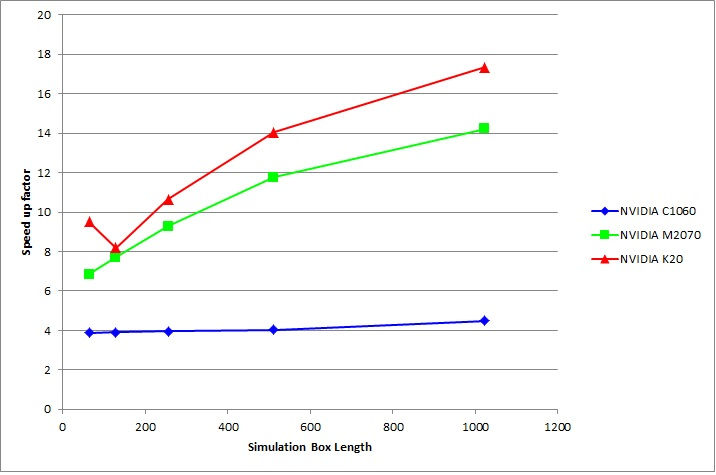
\includegraphics[scale=0.7]{fig10_x5650.JPG}
\caption{Measured speed up factors for the Orszag-Tang test problem performed on different numerical grids, comparing NVIDIA GPUs against the Intel X5650 CPU.}
\end{figure}



%FIGURE 11 here caption: Measured speed up factors for the Orszag-Tang test problem performed on different numerical grids, comparing NVIDIA GPUs against the Intel E5-2670 CPU.\\

\begin{figure}[h]
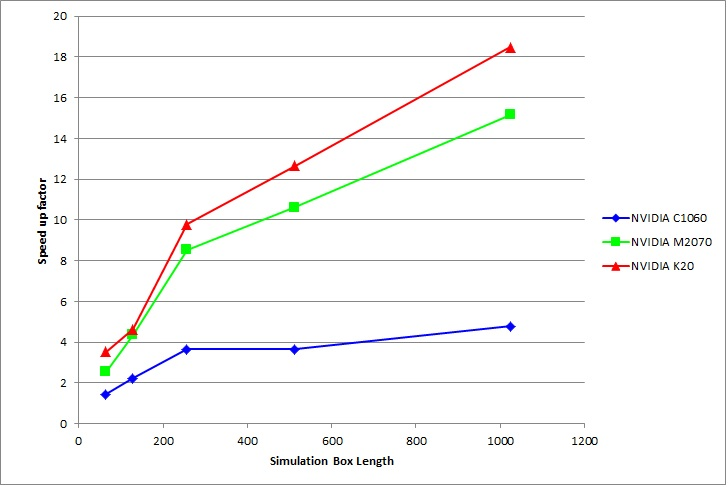
\includegraphics[scale=0.7]{fig11_E5-2670.JPG}
\caption{Measured speed up factors for the Orszag-Tang test problem performed on different numerical grids, comparing NVIDIA GPUs against the Intel E5-2670 CPU.}
\end{figure}







  

%FIGURE 12 here caption: Measured speed up factors for the Orszag-Tang test problems of different the numerical grid size and  comparing NVIDIA GPUs against the fully occupied Intel X5650 CPU.\\

\begin{figure}[h]
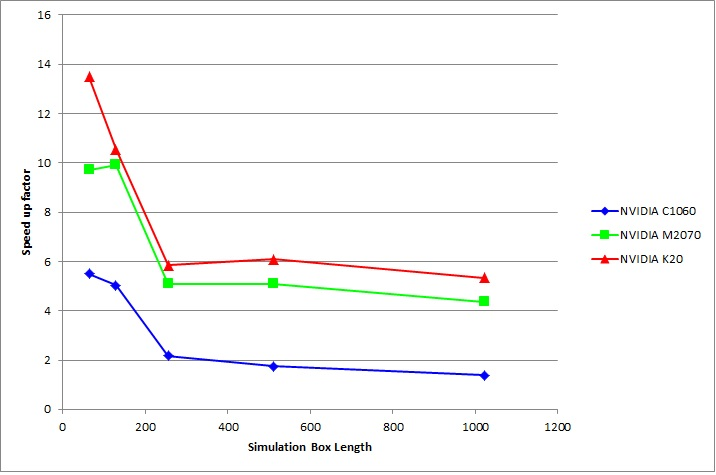
\includegraphics[scale=0.7]{fig12_x5650_6c.JPG}
\caption{Measured speed up factors for the Orszag-Tang test problems of different the numerical grid size and  comparing NVIDIA GPUs against the fully occupied Intel X5650 CPU.}
\end{figure}

%FIGURE 13 here caption: Measured speed up factors for the Orszag-Tang test problems of different sizes of the numerical grid with comparing NVIDIA GPUs against the fully occupied Intel Xeon E5-2670  CPU.\\

\begin{figure}[h]
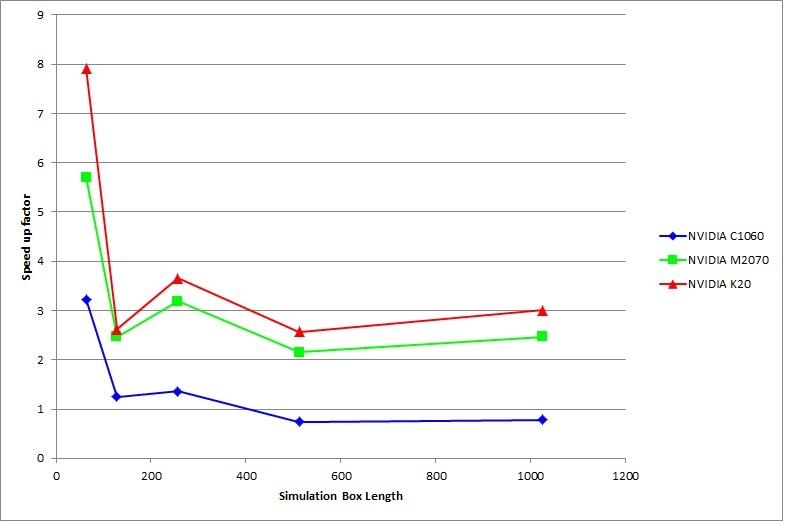
\includegraphics[scale=0.7]{fig13_E5-2670_8c.JPG}
\caption{ Measured speed up factors for the Orszag-Tang test problems of different sizes of the numerical grid with comparing NVIDIA GPUs against the fully occupied Intel Xeon E5-2670  CPU.}
\end{figure}


\section{Conclusions}
We have presented a description of a GPU implementation of a non-linear MHD solver employing artificial numerical diffusion to control numerical instabilities. The code  is developed on the basis of the well-known VAC, (see \citep{Toth et al. 1998} ) and SAC, (see \citep{Shelyag et al. 2008}) platforms. Both of these applications have been tested extensively and provide good agreement with the standard 1-3D HD and MHD tests. The design of the SMAUG implementation has followed that of VAC and SAC very closely. 

The main achievement of SMAUG is the performance benefit which we have demonstrated. This has resulted in a significant cost saving for hardware. To summarise, running the 1024x1024 grid Orszag-Tang problem on a single M2070 GPU is 18 times faster than the same problem running on a single core of an Intel Xeon X5650 CPU. Running the same problem over all 6 cores of the Intel Xeon X5650 reduced the speed-up achieved by the M2070 to a factor of 4. Our results demonstrate that the performance benefits of using a GPU improved as the problem size was increased.

One of the limitations of the current code is related to the problem size. With the 6 GB  of GPU RAM the problem size is limited to a model of 128x128x128 grid points. This will be improved in two ways. Firstly, by making use of MPI to distribute the numerical grid over many GPUs; and, secondly, optimising the usage of temporary data storage employed by SMAUG.  Although we have already successfully scaled the solution to many GPUs, one of the main improvements will be to employ the so-called GPU direct software to enable direct peer-to-peer communications between GPU host memory. 

Further motivations for using GPUs are due to good characteristics of compute performance per unit of power and compute performance per unit of costs. The development roadmap presented by NVIDIA indicates that the Kepler GPU card will aim for 5 double precision gigaflops per watt and the Maxwell GPU will achieve around 15 gigaflops per watt. This represents a 3-fold and 10-fold improvement when compared to the current Fermi GPUs.  Future work will consider the scaling of the performance as SMAUG is used to distribute a problem across multiple GPUs and multiple CPU cores. For this performance assessment it is necessary to evaluate the dependency of the scaling on the different ways of distributing a domain across the processing elements (the GPUs or CPU cores). It is also important to understand how MHD algorithms may best exploit future multi-core processor architectures such as the Intel many integrated core (MIC) architecture or the NVIDIA Maxwell GPU expected in 2015.

The GPU-based algorithm described here, will be used to provide a platform for the simulation of  wave propagation in the strongly stratified and magnetised solar interior and atmosphere. Intial testing has demonstrated that the code is more than able to handle such problems with an excellent agreement compared with the original SAC code of \citep{Shelyag et al. 2008}. For the various complex tests cases which have been considered the results show that the SMAUG successfully reproduces physical processes. Consequently, we are lead to the conclusion that the code can be used as a reliable tool for modelling the physics and perhaps even more importantly prediciting new features of astrophysical plasmas.




\section{Acknowledgement}
MKG acknowledges support from the White Rose Grid e-science centre and funding from the EPSRC contract EP/F057644/1.
MKG acknowledges the support of NVIDIA for allowing testing of the K20 GPU through its early access program and for the donation of a K20 GPU. 
RE acknowledges M. K\'eray for patient encouragement and is also grateful to NSF, Hungary (OTKA, Ref. No. K83133). 
The authors thank the Science and Technology Facilities Council (STFC), UK for the support they received. We acknowledge Anthony Brookfield and Corporate Information and Computing Services at The University of Sheffield for the provision of the High Performance Computing Service.

%http://for.mat.bham.ac.uk/R.W.Kaye/latex/crossref.pdf


%\section{References}
%\bibliographystyle{model1-num-names}
\bibliographystyle{authordate1}
%\bibliographystyle{unsrt}
%\bibliographystyle{plain}
\bibliography{smaug_jaanda_2014}
%\begin{bibliography}{smaug_jaanda_2014}
%\begin{thebibliography}





\end{bibliography}




\appendix
\section{ The Full MHD Equations}

%\appendix\label{B}
%\section{ The Full MHD Equations}\label{A}


%\section*{Appendix A: The Full MHD Equations}
%\refstepcounter{section}
%\label{appendix:a}

 The full MHD equations, including the hyper-diffusion source terms read as
\begin{equation}\label{eqprho}
{{\partial \tilde{\rho}}\over{\partial t}}+\nabla\cdot\left( {\bf v}(\rho_{b} + \tilde{\rho})\right)=0+D_{\rho}(\tilde{\rho}),
\end{equation}




%\begin{equation}\label{eqpmom}
\begin{eqnarray}\label{eqpmom}\nonumber
&&{{\partial [ (\tilde{\rho}+\rho_{b} ) {\bf v}]}\over{\partial t}}+\nabla\cdot\left( {\bf v}(\tilde{\rho} +\rho_{b}){\bf v}-{\bf \tilde{B} \tilde{B}} \right)\\ 
                               && -\nabla [\tilde{\bf B}{\bf B}_{b}+{\bf B}_{b}\tilde{\bf B}] +\nabla \tilde{p}_{t} =\tilde{\rho}{\bf g}+\bf{D}_{\rho v}[(\tilde{\rho }+\rho_{b})\bf v],
\end{eqnarray}
%\end{equation}

%\begin{equation}\label{eqpe}
\begin{eqnarray}\label{eqpe}\nonumber
{{\partial \tilde{e}}\over{\partial t}}+\nabla\cdot\left({\bf v}(\tilde{e}+e_{b})-{\tilde{\bf B} \tilde{\bf B}}\cdot{\bf v}+{\bf v}\tilde{p}_{t}\right)-\nabla [(\tilde{\bf B}{\bf B}_{b}+{\bf B}_{b}\tilde{\bf B})\cdot\bf v]\\
+p_{tb}\nabla {\bf v}-{\bf B}_{b}{\bf B}_{b}\nabla {\bf v}=\tilde{\rho}{\bf g}\cdot{\bf v}+D_{e}(\tilde{e}),
\end{eqnarray}

\begin{equation}\label{eqpb}
{{\partial\tilde{{\bf B}}}\over{\partial t}} +\nabla \cdot\left(  {\bf v}(\tilde{ \bf B} + {\bf B}_b)-(\tilde{ \bf B} + {\bf B}_b){\bf v}\right)=0+\bf{D}_{B}(\tilde{\bf B}),
\end{equation}


where
\begin{equation}\label{eqppt}
\tilde{p}_{t}=\tilde{p}_{k}+{{{\bf B}^{2}}\over{2}}+{\bf B}_{b}\tilde{\bf B},
\end{equation}

\begin{equation}\label{eqppk}
\tilde{p}_{k}=(\gamma -1)\left(\tilde{e}-{{(\rho_{b}+\tilde{\rho}){\bf v}^2}\over{2}}-{\bf B}_{b}\tilde{\bf B}-{{\tilde{\bf B}^{2}}\over{2}}\right),
\end{equation}

\begin{equation}
p_{tb}=p_{kb}+{{{\bf B}_{b}^{2}}\over{2}},
\end{equation}

\begin{equation}\label{eqppkb}
p_{kb}=(\gamma -1)\left(e_{b}-{{{\bf B}_{b}^2}\over{2}}    \right).
\end{equation}

%REV1C1
The MHD equations for momentum \eqref{eqpmom} and energy \eqref{eqpe} are re-ordered by
taking into account the magnetohydrostatic equilibrium condition.  It was found advantageous to use
this, apparently more complex form of the MHD equations for numerical simulations of processes in a gravitationally stratified plasma. The $0+$ term in equation \eqref{eqprho} and  \eqref{eqpb} indicates that the right hand side of these expressions are zero without the inclusion of the numerical diffusion terms. It is important to note that the fully perturbed expressions include diffusive source terms on the right-hand-side. These terms are employed to stabilise the computational solutions using proven hyperdiffusion method, see \citep{Caunt \& Korpi 2001, Stein \& Nordlund 1998}. A helpful discussion of the hyper-diffusion method and its implementation is provided by 
%S$\o$ndergaard and Hansen 
\citep{Sondergaard \& Hansen 1999}.
 The numerical algorithm implemented to solve equations \eqref{eqprho}-\eqref{eqppkb} is based on a fourth order central differencing method for spatial derivatives and a second or fourth order Runge-Kutta solver for the time derivatives. It is important to note that, since we use central differencing, the  quantity $\nabla \cdot \bf B$ is conserved and may be constrained to zero. Schemes preserving the constraint $\nabla \cdot \bf B=0$ have been reviewed by 
%Toth
\citep{Toth 2000)}. The mechanism of hyperdiffusion is used to control the stability of the solutions at discontinuities and shock fronts in equation  \eqref{eqprho} to  \eqref{eqpb}. The additional hyper-diffusive terms for the perturbed density and energy are written as
\begin{equation}\label{eqdifrho}
D_{\rho}=\sum _{i} {{\partial}\over{\partial x_{i}}}\nu _{i}(\rho) {{\partial}\over{\partial x_{i}}}\tilde{\rho}.
\end{equation}
The term $D_{e}$ in the energy equation \eqref{eqpe} consists of three parts:
\begin{equation}\label{eqdife}
D_{e}=D_{e}^{diffusive}+D_{e}^{viscous}+D_{e}^{ohmic},
\end{equation}
which describe thermal diffusion, viscous and ohmic heating of the plasma, respectively
\begin{equation}\label{eqdifedif}
D_{e}^{diffusive}=\sum _{i} {{\partial}\over{\partial x_{i}}}\nu _{i}(e) {{\partial}\over{\partial x_{i}}}\tilde{\epsilon},
\end{equation}
where $\tilde{\epsilon}$ is the thermal energy perturbation
\begin{equation}
\tilde{\epsilon}=\tilde{e}-(\rho_{b}+\tilde{\rho}){{{\bf v}^2}\over{2}}-{{\tilde{\bf B}^{2}}\over{2}}.
\end{equation}
The hyperviscous and ohmic heating terms in\eqref{eqdife} are set as follows:
\begin{equation}
{\bf D}_{e}^{visc}=\nabla \cdot ({\bf v}\cdot \tau )
\end{equation}
and
\begin{equation}
{\bf D}_{e}^{ohmic}=\nabla \cdot ({\bf B}\times \boldsymbol{\varepsilon} ).
\end{equation}
For the vector variables the hyper-diffusive terms are
\begin{equation}
{\bf D}_{\rho \nu}=\nabla \cdot {\bf \tau}
\end{equation}
and
\begin{equation}\label{eqdifb}
{\bf D}_{\bf B}= -\nabla \times {\boldsymbol{ \varepsilon}}.
\end{equation}
Here $ \bf \tau $ is the viscous stress tensor
\begin{equation}
\tau _{kl}={{1}\over{2}}(\tilde{\rho}+\rho _{b})\left[  \nu _{k}(\nu _{l}) {{\partial \nu_{l}}\over{\partial x_{k}}} +    \nu _{l}(\nu _{k}) {{\partial \nu_{k}}\over{\partial x_{l}}}     \right],
\end{equation}
and $  \boldsymbol{\varepsilon} $ is defined by
\begin{equation}
\varepsilon _{k}=\epsilon_{klm}\left[  \nu _{l}(\tilde{B}_{m})  {{\partial \tilde{B}_{m}}\over{\partial x_{l}}} \right],
\end{equation}
where $\epsilon_{klm}$ is the Levi-Civita symbol and a summation of the indices $l$ and $m$ is taken. The hyper-viscosity coefficient for the variable $u$ in the $i^{th}$ direction is
\begin{equation}\label{eqhyp}
\nu _{i}(u)=c_{2}^{u}\Delta x_{i}v_{t}{{max \left| \Delta_i^{3} u\right|}\over{max \left| \Delta _{i}^{1}u\right|}},
\end{equation}
where $v_{t}=v_{a}+v_{s}$ is the sum of the maximum Alfv\'{e}n and sound speeds in the domain, $\Delta^{3}_{i}$ and $\Delta^{1}_{i}$ are forward difference operators  to third and first order, respectively, in the $\it{i}$-th direction. The spatial resolutions are given by $\Delta x_{i}$. The coefficient $c_{2}^{u}$ is set such that it ensures numerical stability of the solution.
The SAC code uses the MPI VAC software as the basis for its implementation \citep{Toth 1996)} that includes the MPI domain decomposition. However, this MPI implementation had to be generalised to include the exchange of the hyper-diffusive contributions for the neighbouring domains. 




%\appendix{B}
\section{ Verification Tests}
%\section{ Verification Tests}\label{B}
%\section*{Appendix B:  Verification Tests}
%\refstepcounter{section}
%\label{appendix:b}

\subsection{Brio \& Wu Shock Tube}
The Brio and Wu  shock tube is a 1D ideal MHD test problem in which the initial conditions of the model feature a discontinuity in the centre of the configuration i.e. the left and right states are initialised to different values at $x=0.5$ (see, \citep{Brio \& Wu 1988}). Either side of the discontinuity the initial parameters are: $p_{l}=1,p_{r}=0.1,\rho_{l}=1,\rho_{r}=0.125,B_{yl}=1,B_{yr}=-1$ $B_{x}=0.75$. Brio and Wu used an upwind differencing scheme and  a linearisation method called the Roe procedure to solve a Riemann-type problem, see \citep{Roe 1981}. The Riemann problem is the solution of a conserved system which has states separated by a discontinuity. In the method employed by Brio and Wu, the exact solution is approximated by a linearised version which is averaged on either side of the discontinuity. Running the problem on a numerical domain with 800 grid points, gives an excellent agreement with the original SAC code results \citep{Shelyag et al 2008}. Figure 14 exhibits features such as the slow compound wave at $x=0.475$, the contact discontiniuity at $x=0.55$, the slow shock at $x=0.65$ and the fast rarefaction at $x=0.85$ are observed. This test ensures the validity of the code by running the numerical simulation along the $\it{x} , \it{y}$ and $\it{z}$ axis in turn. There was found to be no dependency on the orientation of the Brio-Wu and shock tube problem.\\

%FIGURE B1 here caption: A snapshot of the Brio and Wu problem numerical solution taken at time $\it t$=0.1. The density, tangential velocity, %normal velocity and tangential magnetic field are shown respectively.

\begin{figure}[h]
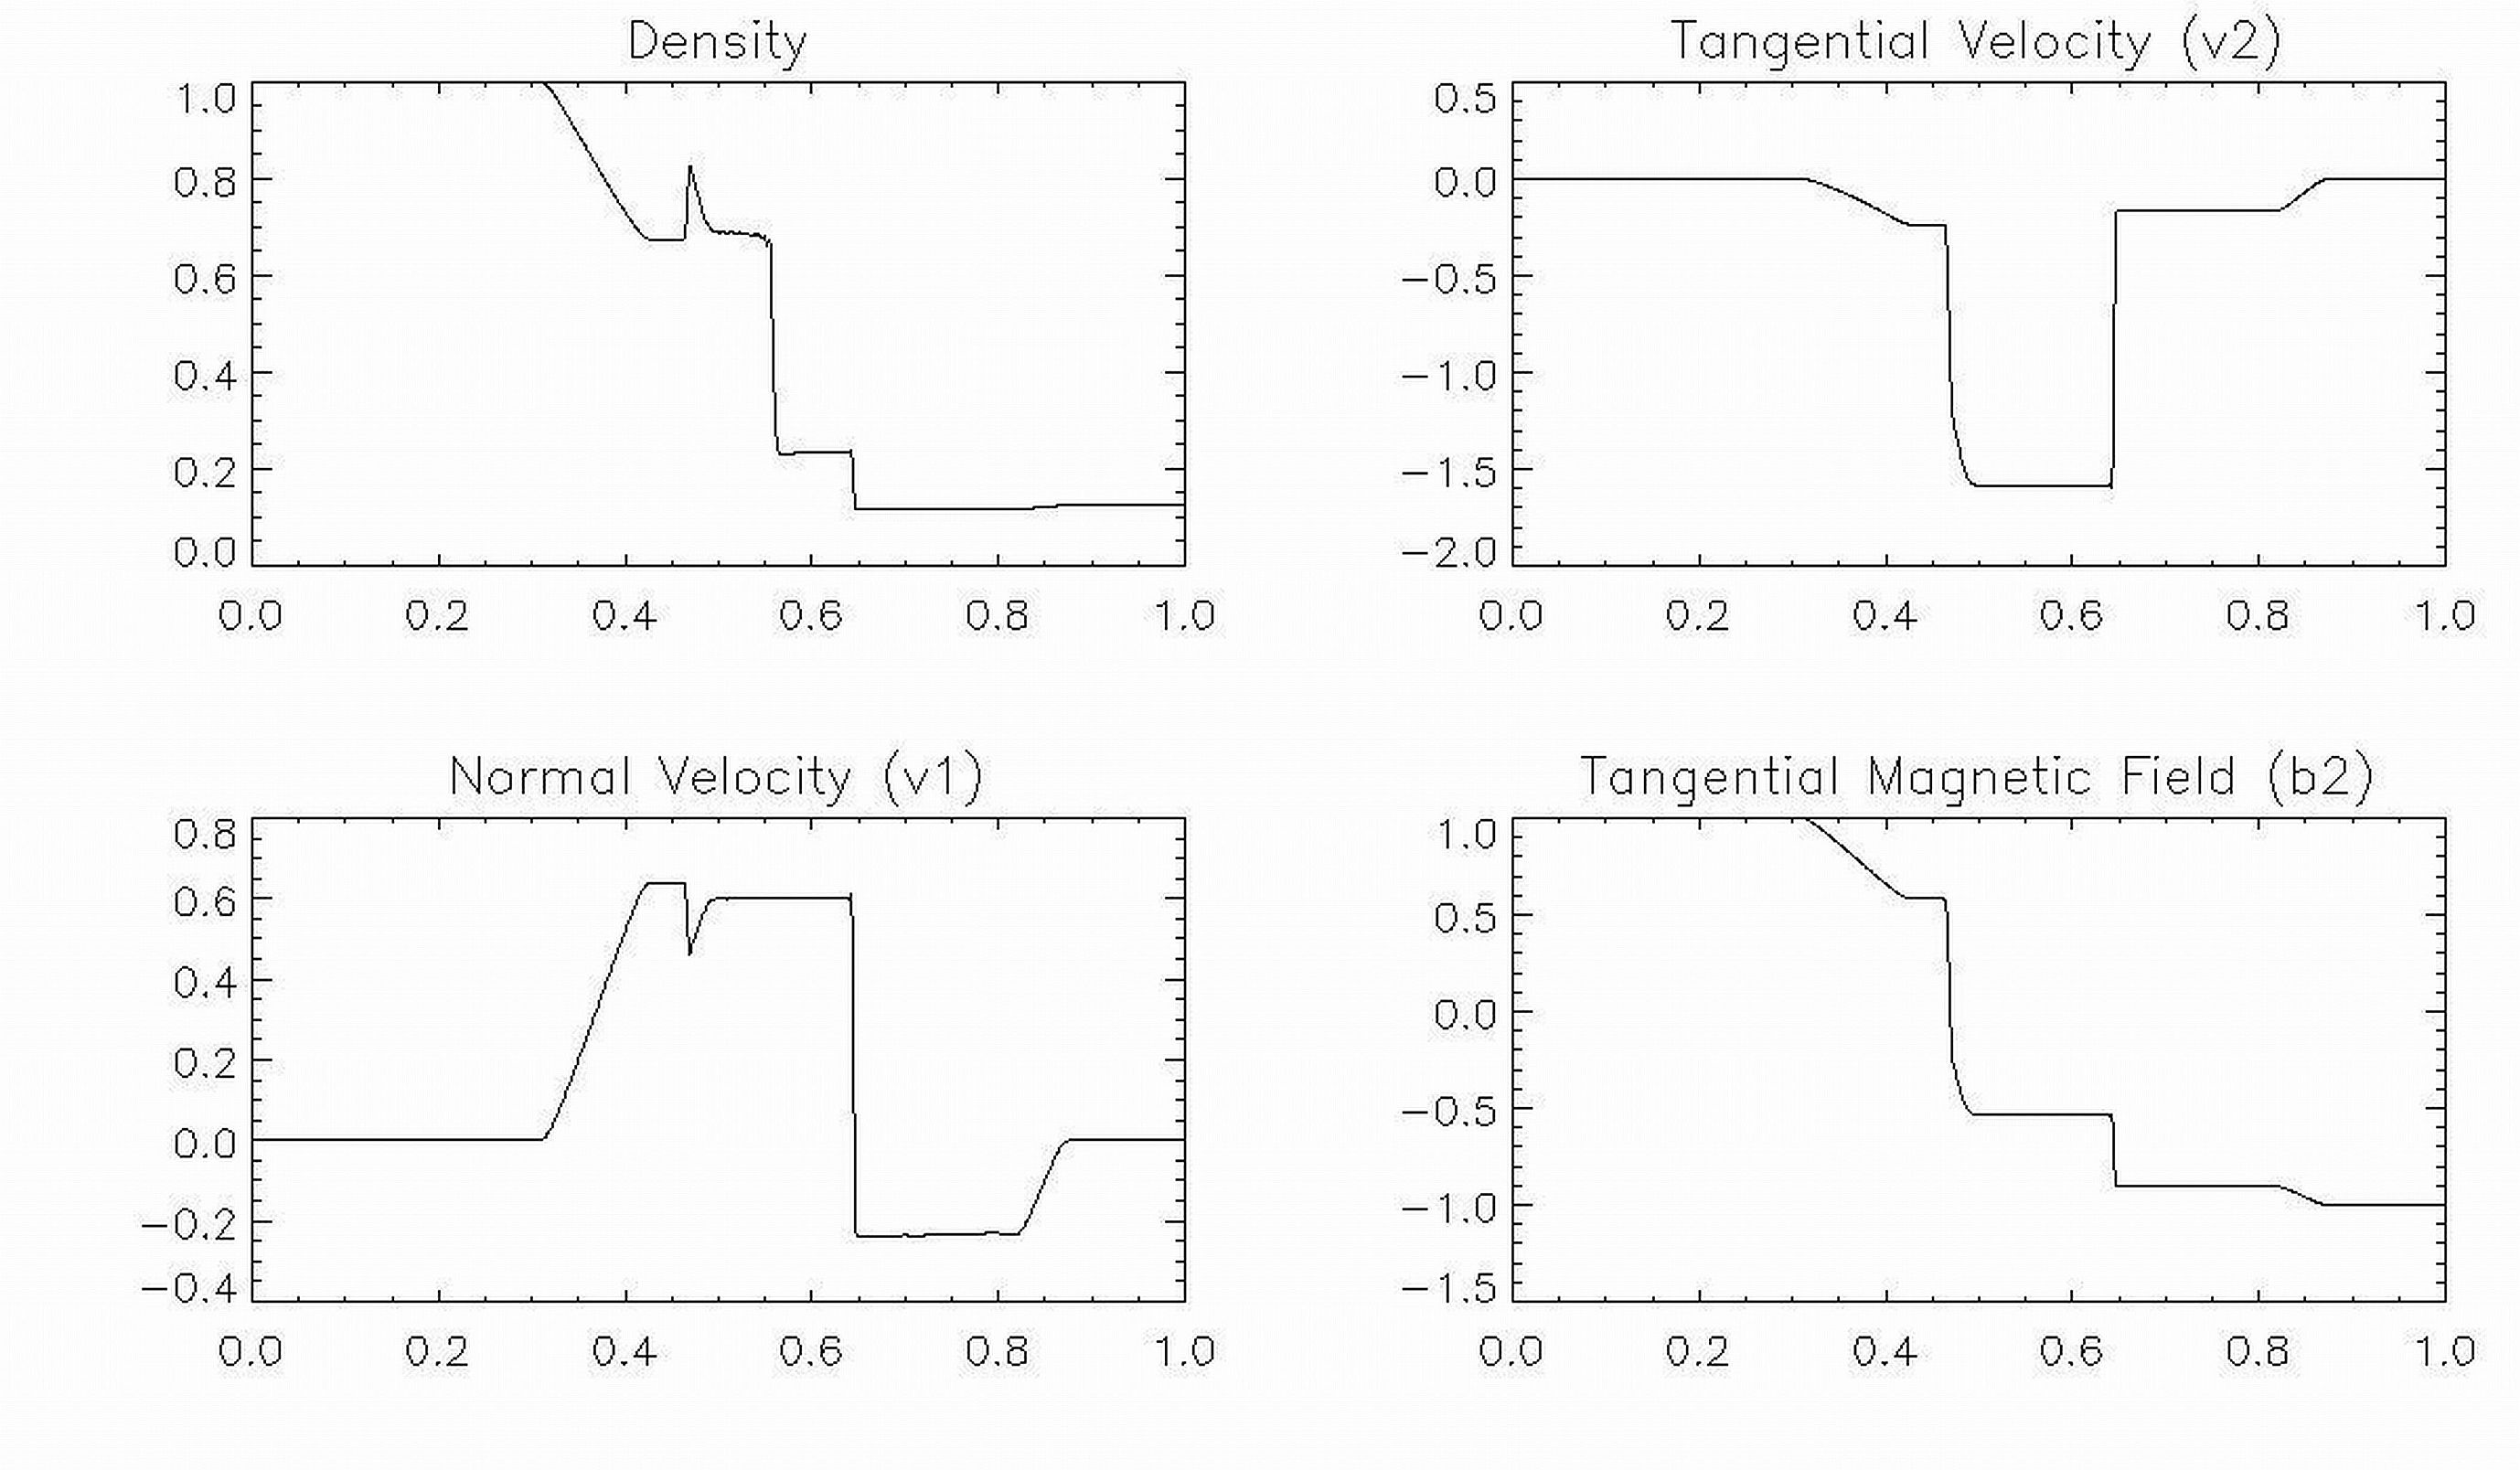
\includegraphics[scale=0.9]{figure_b1_bw.jpg}
\caption{A snapshot of the Brio and Wu problem numerical solution taken at time $\it t$=0.1. The density, tangential velocity, normal velocity and tangential magnetic field are shown.}
\end{figure}





\subsection{Orszag-Tang vortex}
The complexities in the Orszag-Tang vortex present a challenging problem with which the code may be further validated in two dimensional geometry, see \citep{Orszag \& Tang 1979}. The code is required to be sufficiently robust so that it can handle supersonic MHD turbulence. For this test, a 512x512 simulation box was used. The boundaries of the computational  domain were set as periodic. This problem provides an excellent opportunity to test the background terms by assigning the initial density, initial magnetic field and internal energy to the respective background fields.

The density distributions at $t=0.1, 0.26, 0.42$ and $0.58$   generated by SMAUG are shown in Figure 15 and demonstrate a very good and convincing agreement with their counterpart output of SAC \citep{Shelyag et al. 2008}. The results demonstrate the robustness of the code since it is now able to provide well-defined shock fronts.\\ 

%REV1C8
%Figure 4 illustrates the absolute difference between SAC and SMAUG for the density and energy at $t=0.25$ the small errors are seen to arise at the shock boundaries.

%FIGURE B2 here caption: Orszag-Tang vortex problem computed with SMAUG on a 512x512 grid. The denisty distribution at $\it t$=0.1, 0.26, 0.42, 0.58 s is shown (on left top, right top, left lower and right lower panels respectively).\\

\begin{figure}[h]
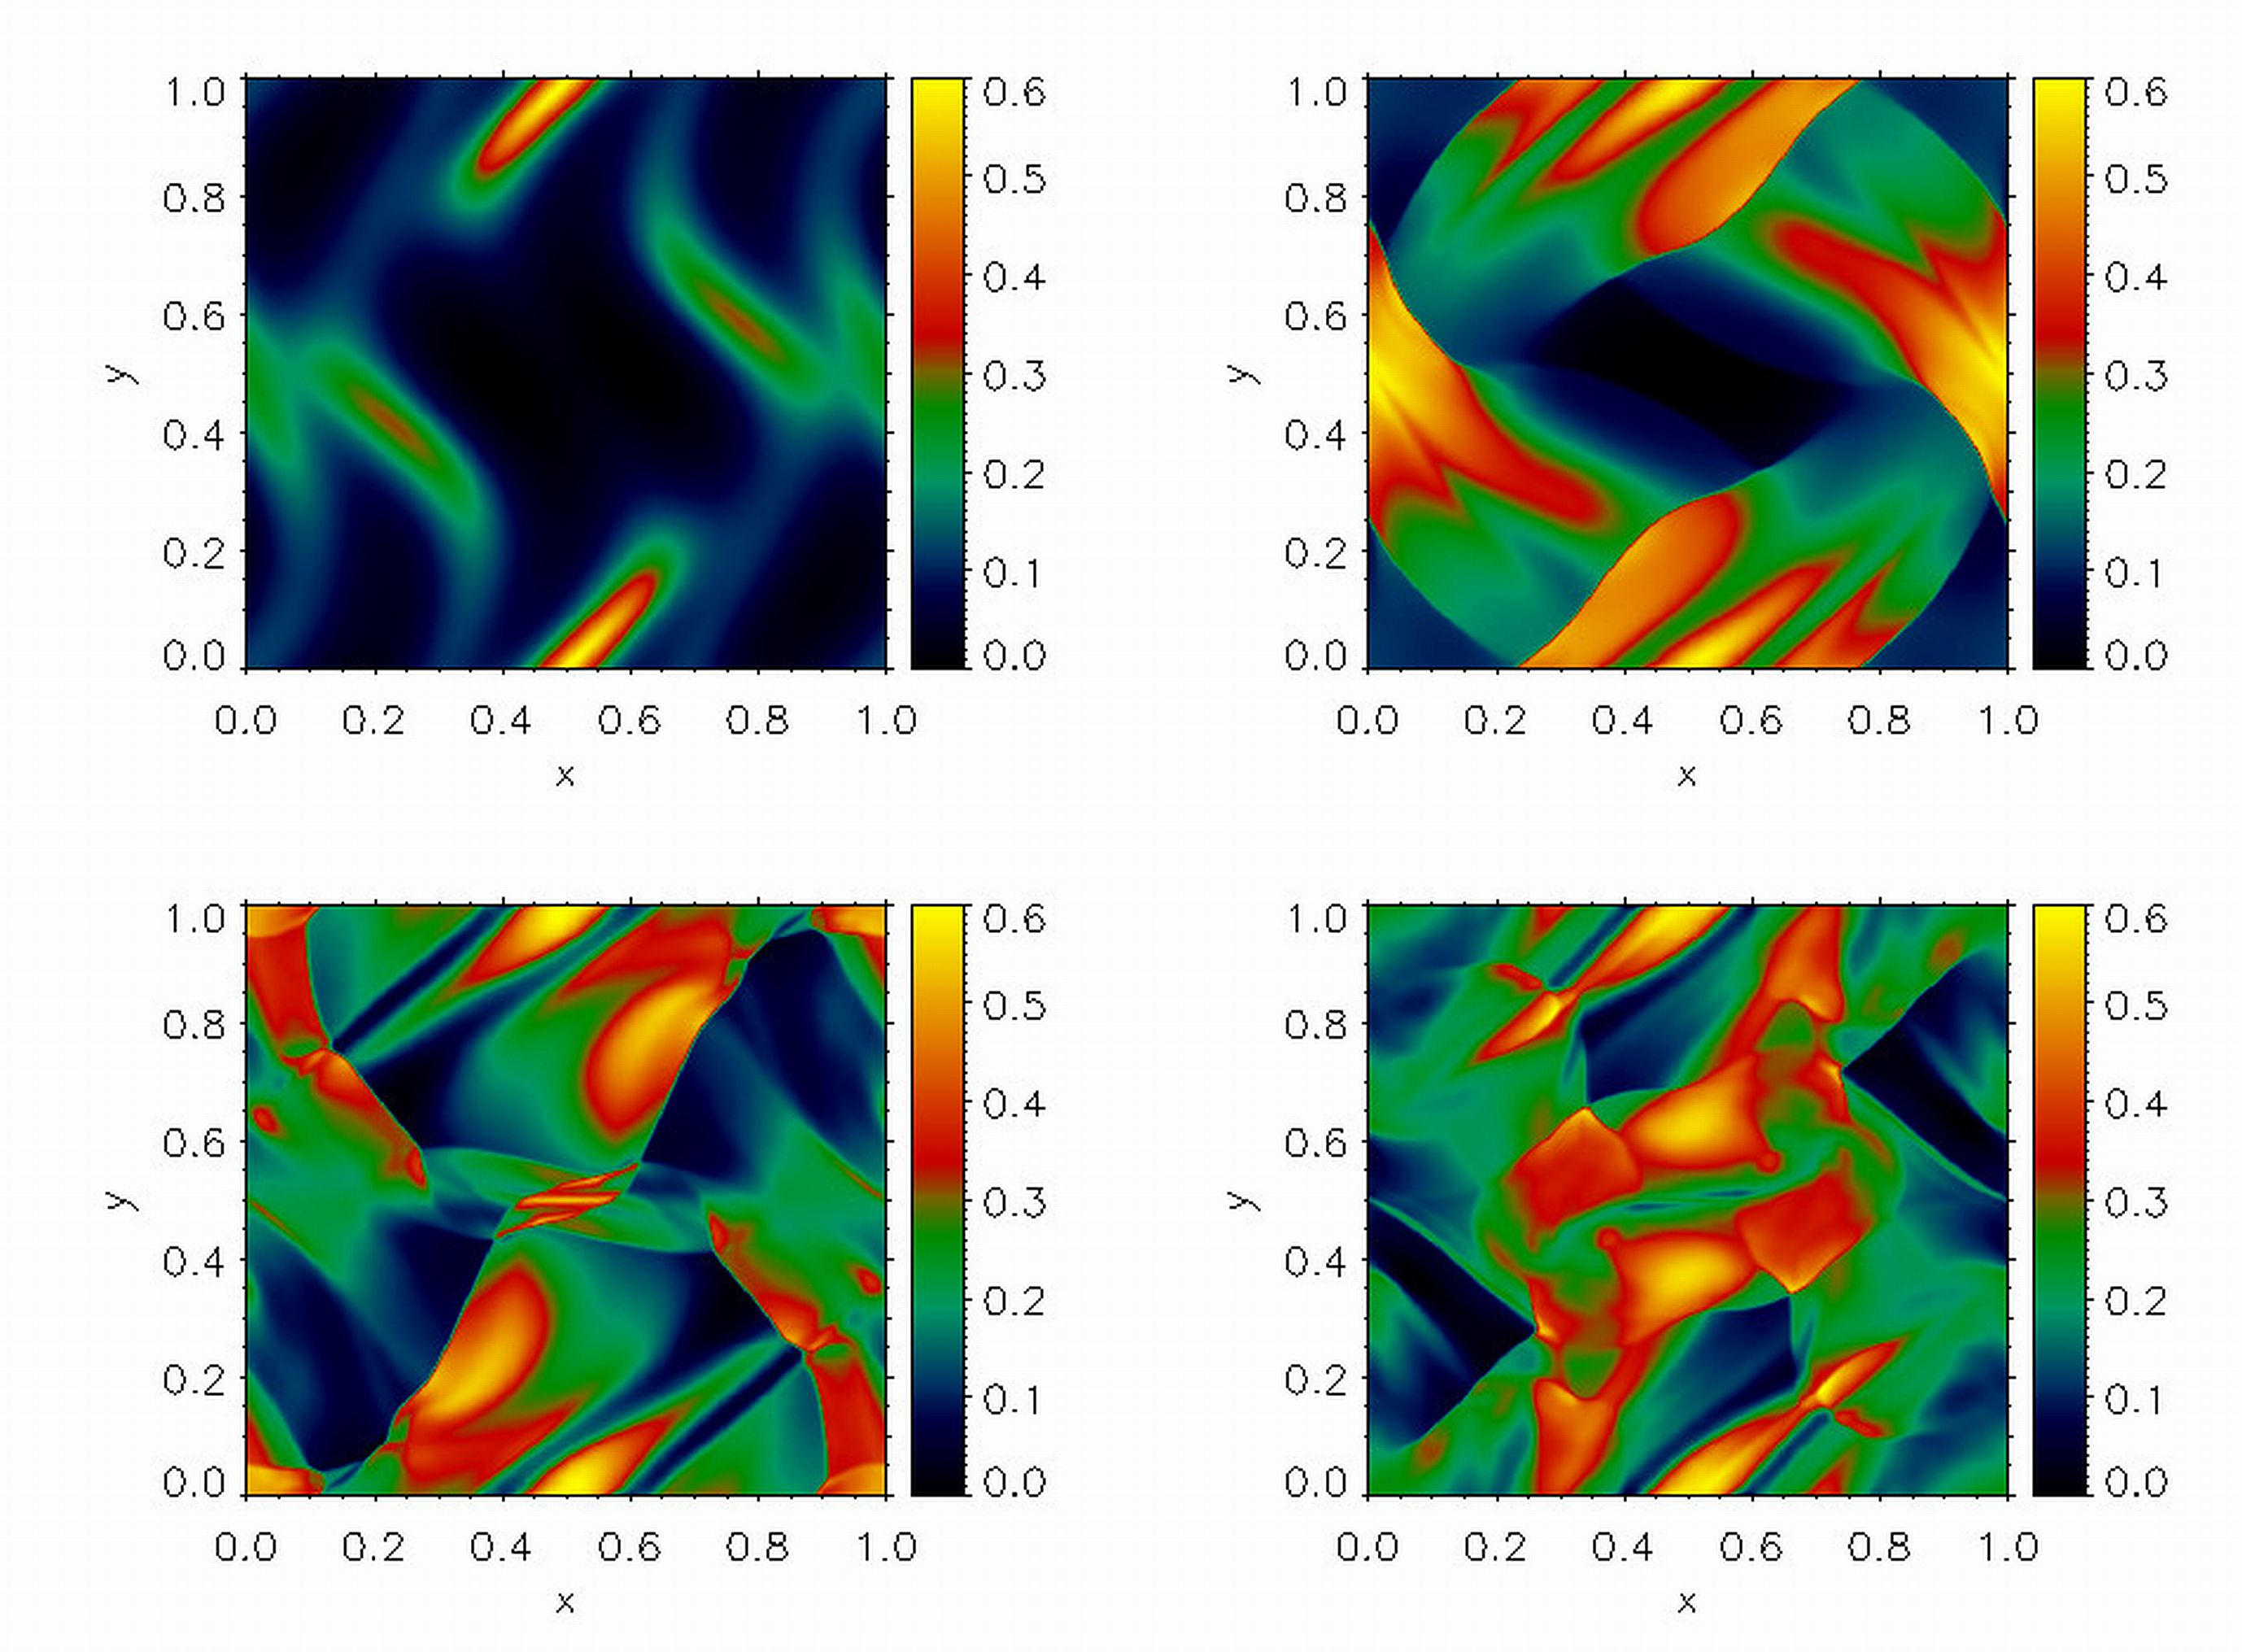
\includegraphics[scale=0.8]{figure_b2_oztdens1.jpg}
\caption{Orszag-Tang vortex problem computed with SAMUG on a 512x512 grid. The denisty distribution at $\it t$=0.1, 0.26, 0.42, 0.58 s is shown (on left top, right top, left lower and right lower panels respectively).}
\end{figure}


%FIGURE B3 here caption: The result of simulation of Sedov blast test problem on 128x128x128 numerical grid with SMAUG. The energy distributions as a function of time are shown at time 1000, 10000, 20000 and 30000 iterations (top left, top right, lower left and lower right) panels respectively.\\



\begin{figure}[]
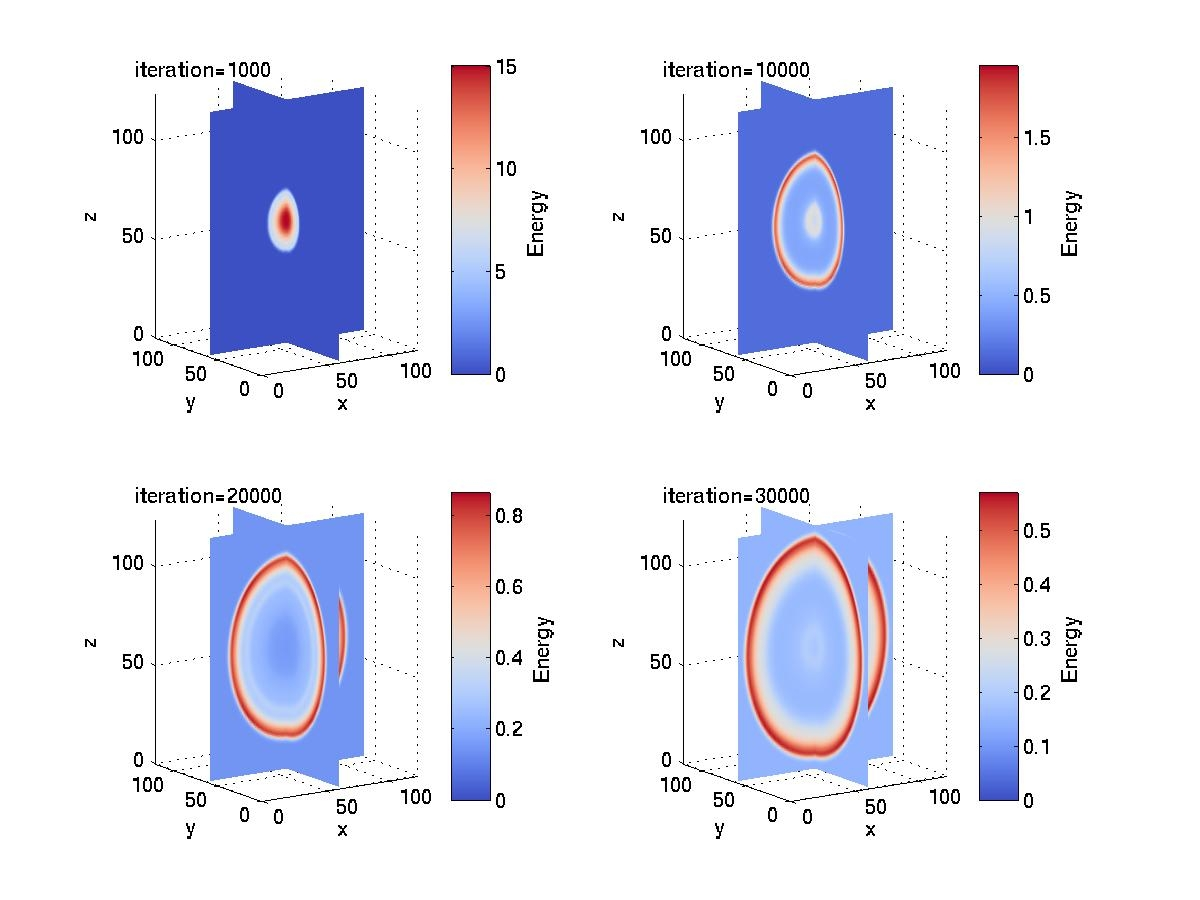
\includegraphics[scale=9.0]{figure_b3_sedov3d_pub.jpg}
\caption{The result of simulation of Sedov blast test problem on 128x128x128 numerical grid with SMAUG. The energy distributions as a function of time are shown at time 1000, 10000, 20000 and 30000 iterations (top left, top right, lower left and lower right) panels respectively.}
\end{figure}







%FIGURE B5 here caption:  Logarithmic plot of the shock front radius of the blast wave as a function of logarithm of time  performed on a 128x128x128 grid with SMAUG (blue diamond shapes) versus the analytical solution (red line).\\

%\begin{figure}[]
%\includegraphics[scale=0.75]{figure8_sedovenergy}
%\caption{Logarithmic plot of the shock front radius of the blast wave as a function of logarithm of time  performed on a 128x128x128 grid with SMAUG %(blue diamond shapes) versus the analytical solution (red line).}
%\end{figure}






\subsection{Blast Waves in 2D and 3D}
This section extends the testing of SMAUG from two-dimensions to a three-dimensional grid with an emphasis on well-characterised blast problems. A blast wave in hydrodynamics is the pressure and flow which results after the release of a highly localised amount of energy. A good astrophysical example is the explosion of a supernova. The comparison between SAC  and SMAUG using blast wave problems was particularly useful for checking the extension of the application from 2D to 3D. Also, by employing the Sedov shock wave we were able to concentrate the hyperdiffusion tests on the momentum terms. Additionally, the Sedov shock wave problem enables a test of the code's capability to model spherically symmetric systems using Cartesian geometry. A solution of the blast wave problem, known as the similarity solution, was developed independently by Taylor \citep{Taylor 1950} and Sedov \citep{Sedov 1946}. The similarity analysis provides a prediction of the radius of the shock front as a function of time i.e.,
\begin{equation}\label{eqblast1}
R(t)=\left({{E}\over{\rho_{0}}}\right)^{{1}\over{5}}t^{{2}\over{5}},
\end{equation}
where $E$ is the energy released by the explosion, $\rho_{0}$  is the density of the surrounding medium. The similarity solution can be derived by starting from the expression for the radius of the shock front as
\begin{equation}\label{eqblast2}
R(t)=E^{\zeta}\rho_{0}^{\eta}t^{\xi}.
\end{equation}
% \eqref{eqblast2} 
By ensuring that both sides of equation 31
have the same dimensions the indices $\zeta$, $\eta$ and $\xi$ can be determined using the similarity solution given by equation 30.  
The simulations were performed using a  128x128x128 numerical domain with a side of length $1.0$ and a surrounding space of uniform density of    $\mathrm{1.0}$. The initial pressure was set to $P=0.1$, however for a shell of radius, $r<0.1$ the pressure was set to 10.0.
The initial velocity was zero and the adiabatic parameter was set to $5/3$.



% This configuration was selected to enable a direct comparison with the results of the A
%\citep{Caunt 2001)}. Figure B4 shows the evolution of the energy distribution as a function of time and illustrates clearly the propagation of the shock front.  
%The simulations were performed using a  128x128x128 numerical domain of side 3.26 light years (i.e. 1 parsec) and a surrounding space of uniform density of    $\mathrm{1.0 kg/m^{3}}$. This configuration was selected to enable a direct comparison with the results of
 %\citep{Caunt 2001)}. Figure 16 shows the evolution of the energy distribution as a function of time and illustrates clearly the propagation of the shock front.  
%REV1C8
%Figure 7  illustrates the absolute difference  between the SAC and SMAUG codes for $\it t$=0.5 My. The greatest errors are to be found at the shock front and the initial source for the explosion, however, even in these regions the level of errors is much smaller than the actual %value predicted by SAC.
%The comparison between the numerical solution  and analytical function B.1 of the shock front radius versus time shows good agreement (see Figure B5).




\end{document}
